	\begin{enumerate}[label=\thesection.\arabic*,ref=\thesection.\theenumi]

\item  
Find four numbers forming a geometric progression in which the third term is greater than the first term by 9, and the second term is greater than the $4^{th}$ by 18.\\
\solution
\input{ncert-maths/11/9/3/21/11.9.3-21.tex}
\pagebreak

\item The $4^{th}$ term of a G.P. is square of its second term, and the first term is -3. Determine its $7^{th}$ term.\\  

\solution 

\iffalse
\let\negmedspace\undefined
\let\negthickspace\undefined
\documentclass[journal,12pt,twocolumn]{IEEEtran}
\usepackage{cite}
\usepackage{amsmath,amssymb,amsfonts,amsthm}
\usepackage{algorithmic}
\usepackage{graphicx}
\usepackage{textcomp}
\usepackage{xcolor}
\usepackage{txfonts}
\usepackage{listings}
\usepackage{enumitem}
\usepackage{mathtools}
\usepackage{gensymb}
\usepackage{comment}
\usepackage[breaklinks=true]{hyperref}
\usepackage{tkz-euclide} 
\usepackage{listings}
\usepackage{gvv}                                        
\def\inputGnumericTable{}                                 
\usepackage[latin1]{inputenc}                                
\usepackage{color}                                            
\usepackage{array}                                            
\usepackage{longtable}                              
\usepackage{calc}                                             
\usepackage{multirow}                                         
\usepackage{hhline}                                           
\usepackage{ifthen}                                           
\usepackage{lscape}

\newtheorem{theorem}{Theorem}[section]
\newtheorem{problem}{Problem}
\newtheorem{proposition}{Proposition}[section]
\newtheorem{lemma}{Lemma}[section]
\newtheorem{corollary}[theorem]{Corollary}
\newtheorem{example}{Example}[section]
\newtheorem{definition}[problem]{Definition}
\newcommand{\BEQA}{\begin{eqnarray}}
\newcommand{\EEQA}{\end{eqnarray}}
\newcommand{\define}{\stackrel{\triangle}{=}}
\theoremstyle{remark}
\newtheorem{rem}{Remark}
\begin{document}

\bibliographystyle{IEEEtran}
\vspace{3cm}

\title{NCERT DISCRETE}
\author{EE23BTECH11214 - Harsha Vardhan Paramata$^{*}$% <-this % stops a space
}
\maketitle
\newpage
\bigskip

\renewcommand{\thefigure}{\theenumi}
\renewcommand{\thetable}{\theenumi}

\textbf{Question 10.5.4.1}:
Which term of the AP: 121, 117, 113, \ldots, is its first negative term?

% Solution
\textbf{Solution}:
\fi
\begin{table}[htbp]
\centering
\begin{tabular}{|l|l|c|}
\hline
\textbf{Symbol} & \textbf{Description} & \textbf{Value} \\
\hline
$x\sbrak{n}$ & General term & \(121 - 4n\) \\
\hline
$x\sbrak{0}$ & Initial term & 121 \\
\hline
$d$ & Common difference & 4 \\
\hline
\end{tabular}

\caption{parameters list}
\end{table}

\begin{align}
x\sbrak{n} &= 121 - 4n < 0 \\
n &> \frac{121}{4} 
\end{align}
The first negative term in the sequence occurs at 
$n = 31$  \\
Z-transform of this sequence:
\begin{align}
    X\brak{z} &= \frac{121 - 125z^{-1}}{1 - 2z^{-1} + z^{-2}}
 ,\quad \abs{z} > \abs{1}
\end{align}
\begin{figure}[!ht] 
\centering
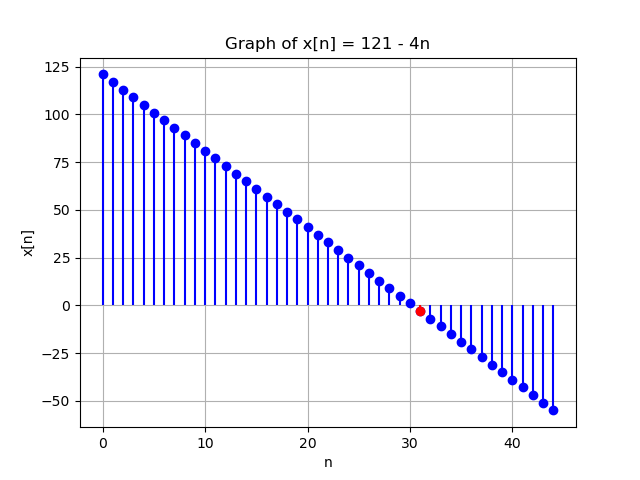
\includegraphics[width=1\columnwidth]{ncert-maths/10/5/4/1/figs/graph.png}
\end{figure}
%\end{document}

\pagebreak

\item Show that
\begin{equation}
    \frac{1\times2^2 + 2\times3^2 + \dots + n\times\brak{n+1}^2}{1^2\times2 + 2^2\times3 +\dots + n^2\times\brak{n+1}}  = \frac{3n+5}{3n+1}\notag
\end{equation}

\solution 

\iffalse
\let\negmedspace\undefined
\let\negthickspace\undefined
\documentclass[journal,12pt,twocolumn]{IEEEtran}
\usepackage{cite}
\usepackage{amsmath,amssymb,amsfonts}
\usepackage{graphicx}
\usepackage{textcomp}
\usepackage{xcolor}
\usepackage{txfonts}
\usepackage{listings}
\usepackage{enumitem}
\usepackage{mathtools}
\usepackage{gensymb}
\usepackage{comment}
\usepackage[breaklinks=true]{hyperref}
\usepackage{tkz-euclide} 
\usepackage{listings}
\usepackage{gvv}                                        
\def\inputGnumericTable{}                                 
\usepackage[latin1]{inputenc}                                
\usepackage{color}                                            
\usepackage{array}                                            
\usepackage{longtable}                                       
\usepackage{calc}                                             
\usepackage{multirow}                                         
\usepackage{hhline}                                           
\usepackage{ifthen}                                           
\usepackage{lscape}
\usepackage[export]{adjustbox}

\newtheorem{theorem}{Theorem}[section]
\newtheorem{problem}{Problem}
\newtheorem{proposition}{Proposition}[section]
\newtheorem{lemma}{Lemma}[section]
\newtheorem{corollary}[theorem]{Corollary}
\newtheorem{example}{Example}[section]
\newtheorem{definition}[problem]{Definition}
\newcommand{\BEQA}{\begin{eqnarray}}
\newcommand{\EEQA}{\end{eqnarray}}
\newcommand{\define}{\stackrel{\triangle}{=}}
\newtheorem{rem}{Remark}

\begin{document}
\parindent 0px
\bibliographystyle{IEEEtran}

\vspace{3cm}
\title{}
\author{EE23BTECH11042 -  Khusinadha Naik$^{*}$
}
\maketitle
\newpage
\bigskip

% \renewcommand{\thefigure}{\theenumi}
% \renewcommand{\thetable}{\theenumi}


\section*{Exercise 9.3}

\noindent \textbf{29.} \hspace{2pt}If A and G be A.M. and G.M., respectively between two positive numbers, prove that the numbers are A $\pm \sqrt{(A+G)(A-G)}$. 

\noindent \textbf{Ans.}\\
\fi

\begin{table}[h]
\centering
\begin{tabular}{|c|c|c|}
        \hline
        \textbf{Parameter} & \textbf{Value} & \textbf{Description} \\
        \hline
        $x_1\brak{n}$ & $\brak{x_1\brak{0}+nd}u\brak{n}$ & AP series \\
	\hline
	$x_2\brak{n}$ & $\brak{x_2\brak{0}\cdot r^{n}}u\brak{n}$ & GP series \\
        \hline
        $x_1\brak{0}, x_2\brak{0}$ & a & First number \\
        \hline
	$x_1\brak{2}, x_2\brak{2}$ & b & Second number \\
	\hline
        $x_1\brak{1}$ & $\brak{x_1\brak{0} + d}u\brak{n} $ & A.M.\brak{A} \\
        \hline
        $x_2\brak{1}$ & $\brak{x_1\brak{0}\cdot r}u\brak{n} $ & G.M.\brak{B} \\
        \hline
\end{tabular}
\caption{Input parameters table}
\label{tab:11.9.3.29.1}

\end{table}

\noindent From \tabref{tab:11.9.3.29.1}
\begin{align}
x_1\brak{2} &= x_2\brak{2} \\
\brak{x_1\brak{0} + 2d }u\brak{n} &= \brak{x_1\brak{0} r^{2}}u\brak{n} \\
2d &= x_1\brak{0}\brak{r^{2} - 1}  \label{eq:11.9.3.29.3}
\end{align}

Now the two numbers are 
\begin{align}
	\brak{a,b} &= \brak{x_1\brak{0}u\brak{n} , \brak{x_1\brak{0} + d} u\brak{n}} \\
&=\brak{x_1\brak{0} + d \pm 2d} u\brak{n} \\
&=\brak{x_1\brak{0} + d \pm \sqrt{d^{2}}} u\brak{n} \\
\notag &=\brak{x_1\brak{0} + d } u\brak{n}\pm\\
& \quad  \sqrt{2x_1\brak{0}d - 2x_1\brak{0}d + d^{2}}  u\brak{n} \label{eq:11.9.3.29.7}
\end{align}

Substituting \eqref{eq:11.9.3.29.3} in \eqref{eq:11.9.3.29.7}:
\begin{align}
\notag (a,b) &= \brak{x_1(0) + d } u\brak{n}\pm \\ 
& \quad \sqrt{2x_1(0)d + x_1(0)  x_1(0)  (1 - r^{2}) + d^{2}} u\brak{n} \\
\notag &= \brak{x_1(0) + d } u\brak{n}\pm \\ 
& \quad \sqrt{x_1(0)^2 + d^2 + 2x_1(0)d - x_1(0)^2r^2} u\brak{n} \\
\notag &= \brak{x_1(0) + d } u\brak{n}\pm \\
& \quad \sqrt{ \brak{\brak{x_1\brak{0} + d} u\brak{n}}^2 - \brak{\brak{x_1\brak{0} r}u\brak{n}}^2}\label{eq:11.9.3.29.10}
\end{align}
\pagebreak

\noindent Comparing \eqref{eq:11.9.3.29.10} , \tabref{tab:11.9.3.29.1} 
\begin{align}
\brak{a,b} =& A \pm \sqrt{A^2 - G^2} \\
\implies \brak{a,b} =& A \pm \sqrt{\brak{A + G}\brak{A - G}}
\end{align}

\begin{align}
u\brak{n} \xleftrightarrow{\mathcal{Z}} &\frac{1}{1 - z^{-1}} \quad , \abs{z} > 1  \label{eq:11.9.3.29.13}\\
nu\brak{n} \xleftrightarrow{\mathcal{Z}} &\frac{z^{-1}}{\brak{1 - z^{-1}}^2} \quad , \abs{z} > 1  \label{eq:11.9.3.29.14}\\
a^{n}u\brak{n} \xleftrightarrow{\mathcal{Z}} &\frac{1}{1 - az^{-1}} \quad , \abs{z} > a \label{eq:11.9.3.29.15}
\end{align}

From  \eqref{eq:11.9.3.29.13} , \eqref{eq:11.9.3.29.14}
\begin{align}
x_1\brak{z} = \frac{x\brak{0}}{1 - z^{-1}} + \frac{dz^{-1}}{\brak{1 - z^{-1}}^2} \quad , \abs{z} > 1 
\end{align}
From \eqref{eq:11.9.3.29.15}
\begin{align}
x_2\brak{z} = \frac{x\brak{0}}{1 - rz^{-1}} \quad , \abs{z} > r
\end{align}




%\end{document}

\pagebreak

\item Write the five terms at n = 1, 2, 3, 4, 5 of the sequence and obtain the Z-transform of the series
\begin{align}
    x \brak{n} &=  -1, & n = 0 \\
    &=   \frac{x \brak{n-1}}{n}, & n > 0\\
    &=   0, & n < 0 
\end{align}

\solution

\iffalse
\let\negmedspace\undefined
\let\negthickspace\undefined
\documentclass[journal,12pt,twocolumn]{IEEEtran}
\usepackage{cite}
\usepackage{amsmath,amssymb,amsfonts}
\usepackage{graphicx}
\usepackage{textcomp}
\usepackage{xcolor}
\usepackage{txfonts}
\usepackage{listings}
\usepackage{enumitem}
\usepackage{mathtools}
\usepackage{gensymb}
\usepackage{comment}
\usepackage[breaklinks=true]{hyperref}
\usepackage{tkz-euclide} 
\usepackage{listings}
\usepackage{gvv}                                        
\def\inputGnumericTable{}                                 
\usepackage[latin1]{inputenc}                                
\usepackage{color}                                            
\usepackage{array}                                            
\usepackage{longtable}                                       
\usepackage{calc}                                             
\usepackage{multirow}                                         
\usepackage{hhline}                                           
\usepackage{ifthen}                                           
\usepackage{lscape}
\usepackage[export]{adjustbox}

\newtheorem{theorem}{Theorem}[section]
\newtheorem{problem}{Problem}
\newtheorem{proposition}{Proposition}[section]
\newtheorem{lemma}{Lemma}[section]
\newtheorem{corollary}[theorem]{Corollary}
\newtheorem{example}{Example}[section]
\newtheorem{definition}[problem]{Definition}
\newcommand{\BEQA}{\begin{eqnarray}}
\newcommand{\EEQA}{\end{eqnarray}}
\newcommand{\define}{\stackrel{\triangle}{=}}
\newtheorem{rem}{Remark}

\begin{document}
\parindent 0px
\bibliographystyle{IEEEtran}

\vspace{3cm}
\title{}
\author{EE23BTECH11042 -  Khusinadha Naik$^{*}$
}
\maketitle
\newpage
\bigskip

% \renewcommand{\thefigure}{\theenumi}
% \renewcommand{\thetable}{\theenumi}


\section*{Exercise 9.3}

\noindent \textbf{29.} \hspace{2pt}If A and G be A.M. and G.M., respectively between two positive numbers, prove that the numbers are A $\pm \sqrt{(A+G)(A-G)}$. 

\noindent \textbf{Ans.}\\
\fi

\begin{table}[h]
\centering
\begin{tabular}{|c|c|c|}
        \hline
        \textbf{Parameter} & \textbf{Value} & \textbf{Description} \\
        \hline
        $x_1\brak{n}$ & $\brak{x_1\brak{0}+nd}u\brak{n}$ & AP series \\
	\hline
	$x_2\brak{n}$ & $\brak{x_2\brak{0}\cdot r^{n}}u\brak{n}$ & GP series \\
        \hline
        $x_1\brak{0}, x_2\brak{0}$ & a & First number \\
        \hline
	$x_1\brak{2}, x_2\brak{2}$ & b & Second number \\
	\hline
        $x_1\brak{1}$ & $\brak{x_1\brak{0} + d}u\brak{n} $ & A.M.\brak{A} \\
        \hline
        $x_2\brak{1}$ & $\brak{x_1\brak{0}\cdot r}u\brak{n} $ & G.M.\brak{B} \\
        \hline
\end{tabular}
\caption{Input parameters table}
\label{tab:11.9.3.29.1}

\end{table}

\noindent From \tabref{tab:11.9.3.29.1}
\begin{align}
x_1\brak{2} &= x_2\brak{2} \\
\brak{x_1\brak{0} + 2d }u\brak{n} &= \brak{x_1\brak{0} r^{2}}u\brak{n} \\
2d &= x_1\brak{0}\brak{r^{2} - 1}  \label{eq:11.9.3.29.3}
\end{align}

Now the two numbers are 
\begin{align}
	\brak{a,b} &= \brak{x_1\brak{0}u\brak{n} , \brak{x_1\brak{0} + d} u\brak{n}} \\
&=\brak{x_1\brak{0} + d \pm 2d} u\brak{n} \\
&=\brak{x_1\brak{0} + d \pm \sqrt{d^{2}}} u\brak{n} \\
\notag &=\brak{x_1\brak{0} + d } u\brak{n}\pm\\
& \quad  \sqrt{2x_1\brak{0}d - 2x_1\brak{0}d + d^{2}}  u\brak{n} \label{eq:11.9.3.29.7}
\end{align}

Substituting \eqref{eq:11.9.3.29.3} in \eqref{eq:11.9.3.29.7}:
\begin{align}
\notag (a,b) &= \brak{x_1(0) + d } u\brak{n}\pm \\ 
& \quad \sqrt{2x_1(0)d + x_1(0)  x_1(0)  (1 - r^{2}) + d^{2}} u\brak{n} \\
\notag &= \brak{x_1(0) + d } u\brak{n}\pm \\ 
& \quad \sqrt{x_1(0)^2 + d^2 + 2x_1(0)d - x_1(0)^2r^2} u\brak{n} \\
\notag &= \brak{x_1(0) + d } u\brak{n}\pm \\
& \quad \sqrt{ \brak{\brak{x_1\brak{0} + d} u\brak{n}}^2 - \brak{\brak{x_1\brak{0} r}u\brak{n}}^2}\label{eq:11.9.3.29.10}
\end{align}
\pagebreak

\noindent Comparing \eqref{eq:11.9.3.29.10} , \tabref{tab:11.9.3.29.1} 
\begin{align}
\brak{a,b} =& A \pm \sqrt{A^2 - G^2} \\
\implies \brak{a,b} =& A \pm \sqrt{\brak{A + G}\brak{A - G}}
\end{align}

\begin{align}
u\brak{n} \xleftrightarrow{\mathcal{Z}} &\frac{1}{1 - z^{-1}} \quad , \abs{z} > 1  \label{eq:11.9.3.29.13}\\
nu\brak{n} \xleftrightarrow{\mathcal{Z}} &\frac{z^{-1}}{\brak{1 - z^{-1}}^2} \quad , \abs{z} > 1  \label{eq:11.9.3.29.14}\\
a^{n}u\brak{n} \xleftrightarrow{\mathcal{Z}} &\frac{1}{1 - az^{-1}} \quad , \abs{z} > a \label{eq:11.9.3.29.15}
\end{align}

From  \eqref{eq:11.9.3.29.13} , \eqref{eq:11.9.3.29.14}
\begin{align}
x_1\brak{z} = \frac{x\brak{0}}{1 - z^{-1}} + \frac{dz^{-1}}{\brak{1 - z^{-1}}^2} \quad , \abs{z} > 1 
\end{align}
From \eqref{eq:11.9.3.29.15}
\begin{align}
x_2\brak{z} = \frac{x\brak{0}}{1 - rz^{-1}} \quad , \abs{z} > r
\end{align}




%\end{document}

\pagebreak


\item Subba Rao started work in 1995 at an annual salary of Rs. 5000 and received an increment of Rs. 200 each year. In which year did his income reach Rs. 7000?

\solution

\iffalse
\let\negmedspace\undefined
\let\negthickspace\undefined
\documentclass[journal,12pt,twocolumn]{IEEEtran}
\usepackage{cite}
\usepackage{amsmath,amssymb,amsfonts}
\usepackage{graphicx}
\usepackage{textcomp}
\usepackage{xcolor}
\usepackage{txfonts}
\usepackage{listings}
\usepackage{enumitem}
\usepackage{mathtools}
\usepackage{gensymb}
\usepackage{comment}
\usepackage[breaklinks=true]{hyperref}
\usepackage{tkz-euclide} 
\usepackage{listings}
\usepackage{gvv}                                        
\def\inputGnumericTable{}                                 
\usepackage[latin1]{inputenc}                                
\usepackage{color}                                            
\usepackage{array}                                            
\usepackage{longtable}                                       
\usepackage{calc}                                             
\usepackage{multirow}                                         
\usepackage{hhline}                                           
\usepackage{ifthen}                                           
\usepackage{lscape}
\usepackage[export]{adjustbox}

\newtheorem{theorem}{Theorem}[section]
\newtheorem{problem}{Problem}
\newtheorem{proposition}{Proposition}[section]
\newtheorem{lemma}{Lemma}[section]
\newtheorem{corollary}[theorem]{Corollary}
\newtheorem{example}{Example}[section]
\newtheorem{definition}[problem]{Definition}
\newcommand{\BEQA}{\begin{eqnarray}}
\newcommand{\EEQA}{\end{eqnarray}}
\newcommand{\define}{\stackrel{\triangle}{=}}
\newtheorem{rem}{Remark}

\begin{document}
\parindent 0px
\bibliographystyle{IEEEtran}

\vspace{3cm}
\title{}
\author{EE23BTECH11042 -  Khusinadha Naik$^{*}$
}
\maketitle
\newpage
\bigskip

% \renewcommand{\thefigure}{\theenumi}
% \renewcommand{\thetable}{\theenumi}


\section*{Exercise 9.3}

\noindent \textbf{29.} \hspace{2pt}If A and G be A.M. and G.M., respectively between two positive numbers, prove that the numbers are A $\pm \sqrt{(A+G)(A-G)}$. 

\noindent \textbf{Ans.}\\
\fi

\begin{table}[h]
\centering
\begin{tabular}{|c|c|c|}
        \hline
        \textbf{Parameter} & \textbf{Value} & \textbf{Description} \\
        \hline
        $x_1\brak{n}$ & $\brak{x_1\brak{0}+nd}u\brak{n}$ & AP series \\
	\hline
	$x_2\brak{n}$ & $\brak{x_2\brak{0}\cdot r^{n}}u\brak{n}$ & GP series \\
        \hline
        $x_1\brak{0}, x_2\brak{0}$ & a & First number \\
        \hline
	$x_1\brak{2}, x_2\brak{2}$ & b & Second number \\
	\hline
        $x_1\brak{1}$ & $\brak{x_1\brak{0} + d}u\brak{n} $ & A.M.\brak{A} \\
        \hline
        $x_2\brak{1}$ & $\brak{x_1\brak{0}\cdot r}u\brak{n} $ & G.M.\brak{B} \\
        \hline
\end{tabular}
\caption{Input parameters table}
\label{tab:11.9.3.29.1}

\end{table}

\noindent From \tabref{tab:11.9.3.29.1}
\begin{align}
x_1\brak{2} &= x_2\brak{2} \\
\brak{x_1\brak{0} + 2d }u\brak{n} &= \brak{x_1\brak{0} r^{2}}u\brak{n} \\
2d &= x_1\brak{0}\brak{r^{2} - 1}  \label{eq:11.9.3.29.3}
\end{align}

Now the two numbers are 
\begin{align}
	\brak{a,b} &= \brak{x_1\brak{0}u\brak{n} , \brak{x_1\brak{0} + d} u\brak{n}} \\
&=\brak{x_1\brak{0} + d \pm 2d} u\brak{n} \\
&=\brak{x_1\brak{0} + d \pm \sqrt{d^{2}}} u\brak{n} \\
\notag &=\brak{x_1\brak{0} + d } u\brak{n}\pm\\
& \quad  \sqrt{2x_1\brak{0}d - 2x_1\brak{0}d + d^{2}}  u\brak{n} \label{eq:11.9.3.29.7}
\end{align}

Substituting \eqref{eq:11.9.3.29.3} in \eqref{eq:11.9.3.29.7}:
\begin{align}
\notag (a,b) &= \brak{x_1(0) + d } u\brak{n}\pm \\ 
& \quad \sqrt{2x_1(0)d + x_1(0)  x_1(0)  (1 - r^{2}) + d^{2}} u\brak{n} \\
\notag &= \brak{x_1(0) + d } u\brak{n}\pm \\ 
& \quad \sqrt{x_1(0)^2 + d^2 + 2x_1(0)d - x_1(0)^2r^2} u\brak{n} \\
\notag &= \brak{x_1(0) + d } u\brak{n}\pm \\
& \quad \sqrt{ \brak{\brak{x_1\brak{0} + d} u\brak{n}}^2 - \brak{\brak{x_1\brak{0} r}u\brak{n}}^2}\label{eq:11.9.3.29.10}
\end{align}
\pagebreak

\noindent Comparing \eqref{eq:11.9.3.29.10} , \tabref{tab:11.9.3.29.1} 
\begin{align}
\brak{a,b} =& A \pm \sqrt{A^2 - G^2} \\
\implies \brak{a,b} =& A \pm \sqrt{\brak{A + G}\brak{A - G}}
\end{align}

\begin{align}
u\brak{n} \xleftrightarrow{\mathcal{Z}} &\frac{1}{1 - z^{-1}} \quad , \abs{z} > 1  \label{eq:11.9.3.29.13}\\
nu\brak{n} \xleftrightarrow{\mathcal{Z}} &\frac{z^{-1}}{\brak{1 - z^{-1}}^2} \quad , \abs{z} > 1  \label{eq:11.9.3.29.14}\\
a^{n}u\brak{n} \xleftrightarrow{\mathcal{Z}} &\frac{1}{1 - az^{-1}} \quad , \abs{z} > a \label{eq:11.9.3.29.15}
\end{align}

From  \eqref{eq:11.9.3.29.13} , \eqref{eq:11.9.3.29.14}
\begin{align}
x_1\brak{z} = \frac{x\brak{0}}{1 - z^{-1}} + \frac{dz^{-1}}{\brak{1 - z^{-1}}^2} \quad , \abs{z} > 1 
\end{align}
From \eqref{eq:11.9.3.29.15}
\begin{align}
x_2\brak{z} = \frac{x\brak{0}}{1 - rz^{-1}} \quad , \abs{z} > r
\end{align}




%\end{document}


\item Consider the sequence whose $n^\text{th}$ term is given by \(2^n\). Find the first 6 terms of this sequence.

\solution

\input{ncert-maths/11/9/1/3/2.tex}

\item If the sum of first 7 terms of an AP is 49 and that of 17 terms is 289, find the sum of first n terms.

\solution

\iffalse
\let\negmedspace\undefined
\let\negthickspace\undefined
\documentclass[journal,12pt,twocolumn]{IEEEtran}
\usepackage{cite}
\usepackage{amsmath,amssymb,amsfonts}
\usepackage{graphicx}
\usepackage{textcomp}
\usepackage{xcolor}
\usepackage{txfonts}
\usepackage{listings}
\usepackage{enumitem}
\usepackage{mathtools}
\usepackage{gensymb}
\usepackage{comment}
\usepackage[breaklinks=true]{hyperref}
\usepackage{tkz-euclide} 
\usepackage{listings}
\usepackage{gvv}                                        
\def\inputGnumericTable{}                                 
\usepackage[latin1]{inputenc}                                
\usepackage{color}                                            
\usepackage{array}                                            
\usepackage{longtable}                                       
\usepackage{calc}                                             
\usepackage{multirow}                                         
\usepackage{hhline}                                           
\usepackage{ifthen}                                           
\usepackage{lscape}
\usepackage[export]{adjustbox}

\newtheorem{theorem}{Theorem}[section]
\newtheorem{problem}{Problem}
\newtheorem{proposition}{Proposition}[section]
\newtheorem{lemma}{Lemma}[section]
\newtheorem{corollary}[theorem]{Corollary}
\newtheorem{example}{Example}[section]
\newtheorem{definition}[problem]{Definition}
\newcommand{\BEQA}{\begin{eqnarray}}
\newcommand{\EEQA}{\end{eqnarray}}
\newcommand{\define}{\stackrel{\triangle}{=}}
\newtheorem{rem}{Remark}

\begin{document}
\parindent 0px
\bibliographystyle{IEEEtran}

\vspace{3cm}
\title{}
\author{EE23BTECH11042 -  Khusinadha Naik$^{*}$
}
\maketitle
\newpage
\bigskip

% \renewcommand{\thefigure}{\theenumi}
% \renewcommand{\thetable}{\theenumi}


\section*{Exercise 9.3}

\noindent \textbf{29.} \hspace{2pt}If A and G be A.M. and G.M., respectively between two positive numbers, prove that the numbers are A $\pm \sqrt{(A+G)(A-G)}$. 

\noindent \textbf{Ans.}\\
\fi

\begin{table}[h]
\centering
\begin{tabular}{|c|c|c|}
        \hline
        \textbf{Parameter} & \textbf{Value} & \textbf{Description} \\
        \hline
        $x_1\brak{n}$ & $\brak{x_1\brak{0}+nd}u\brak{n}$ & AP series \\
	\hline
	$x_2\brak{n}$ & $\brak{x_2\brak{0}\cdot r^{n}}u\brak{n}$ & GP series \\
        \hline
        $x_1\brak{0}, x_2\brak{0}$ & a & First number \\
        \hline
	$x_1\brak{2}, x_2\brak{2}$ & b & Second number \\
	\hline
        $x_1\brak{1}$ & $\brak{x_1\brak{0} + d}u\brak{n} $ & A.M.\brak{A} \\
        \hline
        $x_2\brak{1}$ & $\brak{x_1\brak{0}\cdot r}u\brak{n} $ & G.M.\brak{B} \\
        \hline
\end{tabular}
\caption{Input parameters table}
\label{tab:11.9.3.29.1}

\end{table}

\noindent From \tabref{tab:11.9.3.29.1}
\begin{align}
x_1\brak{2} &= x_2\brak{2} \\
\brak{x_1\brak{0} + 2d }u\brak{n} &= \brak{x_1\brak{0} r^{2}}u\brak{n} \\
2d &= x_1\brak{0}\brak{r^{2} - 1}  \label{eq:11.9.3.29.3}
\end{align}

Now the two numbers are 
\begin{align}
	\brak{a,b} &= \brak{x_1\brak{0}u\brak{n} , \brak{x_1\brak{0} + d} u\brak{n}} \\
&=\brak{x_1\brak{0} + d \pm 2d} u\brak{n} \\
&=\brak{x_1\brak{0} + d \pm \sqrt{d^{2}}} u\brak{n} \\
\notag &=\brak{x_1\brak{0} + d } u\brak{n}\pm\\
& \quad  \sqrt{2x_1\brak{0}d - 2x_1\brak{0}d + d^{2}}  u\brak{n} \label{eq:11.9.3.29.7}
\end{align}

Substituting \eqref{eq:11.9.3.29.3} in \eqref{eq:11.9.3.29.7}:
\begin{align}
\notag (a,b) &= \brak{x_1(0) + d } u\brak{n}\pm \\ 
& \quad \sqrt{2x_1(0)d + x_1(0)  x_1(0)  (1 - r^{2}) + d^{2}} u\brak{n} \\
\notag &= \brak{x_1(0) + d } u\brak{n}\pm \\ 
& \quad \sqrt{x_1(0)^2 + d^2 + 2x_1(0)d - x_1(0)^2r^2} u\brak{n} \\
\notag &= \brak{x_1(0) + d } u\brak{n}\pm \\
& \quad \sqrt{ \brak{\brak{x_1\brak{0} + d} u\brak{n}}^2 - \brak{\brak{x_1\brak{0} r}u\brak{n}}^2}\label{eq:11.9.3.29.10}
\end{align}
\pagebreak

\noindent Comparing \eqref{eq:11.9.3.29.10} , \tabref{tab:11.9.3.29.1} 
\begin{align}
\brak{a,b} =& A \pm \sqrt{A^2 - G^2} \\
\implies \brak{a,b} =& A \pm \sqrt{\brak{A + G}\brak{A - G}}
\end{align}

\begin{align}
u\brak{n} \xleftrightarrow{\mathcal{Z}} &\frac{1}{1 - z^{-1}} \quad , \abs{z} > 1  \label{eq:11.9.3.29.13}\\
nu\brak{n} \xleftrightarrow{\mathcal{Z}} &\frac{z^{-1}}{\brak{1 - z^{-1}}^2} \quad , \abs{z} > 1  \label{eq:11.9.3.29.14}\\
a^{n}u\brak{n} \xleftrightarrow{\mathcal{Z}} &\frac{1}{1 - az^{-1}} \quad , \abs{z} > a \label{eq:11.9.3.29.15}
\end{align}

From  \eqref{eq:11.9.3.29.13} , \eqref{eq:11.9.3.29.14}
\begin{align}
x_1\brak{z} = \frac{x\brak{0}}{1 - z^{-1}} + \frac{dz^{-1}}{\brak{1 - z^{-1}}^2} \quad , \abs{z} > 1 
\end{align}
From \eqref{eq:11.9.3.29.15}
\begin{align}
x_2\brak{z} = \frac{x\brak{0}}{1 - rz^{-1}} \quad , \abs{z} > r
\end{align}




%\end{document}

\pagebreak

\item Write the first five terms of the sequence and obtain the corresponding series:\\
$a_1=a_2=2,$ $a_n=a_{n-1} -1,$ $n>2$\\
\solution
\iffalse
\let\negmedspace\undefined
\let\negthickspace\undefined
\documentclass[journal,12pt,twocolumn]{IEEEtran}
\usepackage{cite}
\usepackage{amsmath,amssymb,amsfonts}
\usepackage{graphicx}
\usepackage{textcomp}
\usepackage{xcolor}
\usepackage{txfonts}
\usepackage{listings}
\usepackage{enumitem}
\usepackage{mathtools}
\usepackage{gensymb}
\usepackage{comment}
\usepackage[breaklinks=true]{hyperref}
\usepackage{tkz-euclide} 
\usepackage{listings}
\usepackage{gvv}                                        
\def\inputGnumericTable{}                                 
\usepackage[latin1]{inputenc}                                
\usepackage{color}                                            
\usepackage{array}                                            
\usepackage{longtable}                                       
\usepackage{calc}                                             
\usepackage{multirow}                                         
\usepackage{hhline}                                           
\usepackage{ifthen}                                           
\usepackage{lscape}
\usepackage[export]{adjustbox}

\newtheorem{theorem}{Theorem}[section]
\newtheorem{problem}{Problem}
\newtheorem{proposition}{Proposition}[section]
\newtheorem{lemma}{Lemma}[section]
\newtheorem{corollary}[theorem]{Corollary}
\newtheorem{example}{Example}[section]
\newtheorem{definition}[problem]{Definition}
\newcommand{\BEQA}{\begin{eqnarray}}
\newcommand{\EEQA}{\end{eqnarray}}
\newcommand{\define}{\stackrel{\triangle}{=}}
\newtheorem{rem}{Remark}

\begin{document}
\parindent 0px
\bibliographystyle{IEEEtran}

\vspace{3cm}
\title{}
\author{EE23BTECH11042 -  Khusinadha Naik$^{*}$
}
\maketitle
\newpage
\bigskip

% \renewcommand{\thefigure}{\theenumi}
% \renewcommand{\thetable}{\theenumi}


\section*{Exercise 9.3}

\noindent \textbf{29.} \hspace{2pt}If A and G be A.M. and G.M., respectively between two positive numbers, prove that the numbers are A $\pm \sqrt{(A+G)(A-G)}$. 

\noindent \textbf{Ans.}\\
\fi

\begin{table}[h]
\centering
\begin{tabular}{|c|c|c|}
        \hline
        \textbf{Parameter} & \textbf{Value} & \textbf{Description} \\
        \hline
        $x_1\brak{n}$ & $\brak{x_1\brak{0}+nd}u\brak{n}$ & AP series \\
	\hline
	$x_2\brak{n}$ & $\brak{x_2\brak{0}\cdot r^{n}}u\brak{n}$ & GP series \\
        \hline
        $x_1\brak{0}, x_2\brak{0}$ & a & First number \\
        \hline
	$x_1\brak{2}, x_2\brak{2}$ & b & Second number \\
	\hline
        $x_1\brak{1}$ & $\brak{x_1\brak{0} + d}u\brak{n} $ & A.M.\brak{A} \\
        \hline
        $x_2\brak{1}$ & $\brak{x_1\brak{0}\cdot r}u\brak{n} $ & G.M.\brak{B} \\
        \hline
\end{tabular}
\caption{Input parameters table}
\label{tab:11.9.3.29.1}

\end{table}

\noindent From \tabref{tab:11.9.3.29.1}
\begin{align}
x_1\brak{2} &= x_2\brak{2} \\
\brak{x_1\brak{0} + 2d }u\brak{n} &= \brak{x_1\brak{0} r^{2}}u\brak{n} \\
2d &= x_1\brak{0}\brak{r^{2} - 1}  \label{eq:11.9.3.29.3}
\end{align}

Now the two numbers are 
\begin{align}
	\brak{a,b} &= \brak{x_1\brak{0}u\brak{n} , \brak{x_1\brak{0} + d} u\brak{n}} \\
&=\brak{x_1\brak{0} + d \pm 2d} u\brak{n} \\
&=\brak{x_1\brak{0} + d \pm \sqrt{d^{2}}} u\brak{n} \\
\notag &=\brak{x_1\brak{0} + d } u\brak{n}\pm\\
& \quad  \sqrt{2x_1\brak{0}d - 2x_1\brak{0}d + d^{2}}  u\brak{n} \label{eq:11.9.3.29.7}
\end{align}

Substituting \eqref{eq:11.9.3.29.3} in \eqref{eq:11.9.3.29.7}:
\begin{align}
\notag (a,b) &= \brak{x_1(0) + d } u\brak{n}\pm \\ 
& \quad \sqrt{2x_1(0)d + x_1(0)  x_1(0)  (1 - r^{2}) + d^{2}} u\brak{n} \\
\notag &= \brak{x_1(0) + d } u\brak{n}\pm \\ 
& \quad \sqrt{x_1(0)^2 + d^2 + 2x_1(0)d - x_1(0)^2r^2} u\brak{n} \\
\notag &= \brak{x_1(0) + d } u\brak{n}\pm \\
& \quad \sqrt{ \brak{\brak{x_1\brak{0} + d} u\brak{n}}^2 - \brak{\brak{x_1\brak{0} r}u\brak{n}}^2}\label{eq:11.9.3.29.10}
\end{align}
\pagebreak

\noindent Comparing \eqref{eq:11.9.3.29.10} , \tabref{tab:11.9.3.29.1} 
\begin{align}
\brak{a,b} =& A \pm \sqrt{A^2 - G^2} \\
\implies \brak{a,b} =& A \pm \sqrt{\brak{A + G}\brak{A - G}}
\end{align}

\begin{align}
u\brak{n} \xleftrightarrow{\mathcal{Z}} &\frac{1}{1 - z^{-1}} \quad , \abs{z} > 1  \label{eq:11.9.3.29.13}\\
nu\brak{n} \xleftrightarrow{\mathcal{Z}} &\frac{z^{-1}}{\brak{1 - z^{-1}}^2} \quad , \abs{z} > 1  \label{eq:11.9.3.29.14}\\
a^{n}u\brak{n} \xleftrightarrow{\mathcal{Z}} &\frac{1}{1 - az^{-1}} \quad , \abs{z} > a \label{eq:11.9.3.29.15}
\end{align}

From  \eqref{eq:11.9.3.29.13} , \eqref{eq:11.9.3.29.14}
\begin{align}
x_1\brak{z} = \frac{x\brak{0}}{1 - z^{-1}} + \frac{dz^{-1}}{\brak{1 - z^{-1}}^2} \quad , \abs{z} > 1 
\end{align}
From \eqref{eq:11.9.3.29.15}
\begin{align}
x_2\brak{z} = \frac{x\brak{0}}{1 - rz^{-1}} \quad , \abs{z} > r
\end{align}




%\end{document}

\pagebreak
\item Insert two numbers between 3 and 81 so that the resulting sequence is G.P.\\

\solution
\input{ncert-maths/11/9/3/26/asnmt1.tex}
\pagebreak

\item  What will Rs 500 amounts to in 10 years after its deposit in a bank which pays annual interest rate of 10$\%$ compounded annually?

\solution
    \iffalse
\let\negmedspace\undefined
\let\negthickspace\undefined
\documentclass[journal,12pt,twocolumn]{IEEEtran}
\usepackage{cite}
\usepackage{amsmath,amssymb,amsfonts}
\usepackage{graphicx}
\usepackage{textcomp}
\usepackage{xcolor}
\usepackage{txfonts}
\usepackage{listings}
\usepackage{enumitem}
\usepackage{mathtools}
\usepackage{gensymb}
\usepackage{comment}
\usepackage[breaklinks=true]{hyperref}
\usepackage{tkz-euclide} 
\usepackage{listings}
\usepackage{gvv}                                        
\def\inputGnumericTable{}                                 
\usepackage[latin1]{inputenc}                                
\usepackage{color}                                            
\usepackage{array}                                            
\usepackage{longtable}                                       
\usepackage{calc}                                             
\usepackage{multirow}                                         
\usepackage{hhline}                                           
\usepackage{ifthen}                                           
\usepackage{lscape}
\usepackage[export]{adjustbox}

\newtheorem{theorem}{Theorem}[section]
\newtheorem{problem}{Problem}
\newtheorem{proposition}{Proposition}[section]
\newtheorem{lemma}{Lemma}[section]
\newtheorem{corollary}[theorem]{Corollary}
\newtheorem{example}{Example}[section]
\newtheorem{definition}[problem]{Definition}
\newcommand{\BEQA}{\begin{eqnarray}}
\newcommand{\EEQA}{\end{eqnarray}}
\newcommand{\define}{\stackrel{\triangle}{=}}
\newtheorem{rem}{Remark}

\begin{document}
\parindent 0px
\bibliographystyle{IEEEtran}

\vspace{3cm}
\title{}
\author{EE23BTECH11042 -  Khusinadha Naik$^{*}$
}
\maketitle
\newpage
\bigskip

% \renewcommand{\thefigure}{\theenumi}
% \renewcommand{\thetable}{\theenumi}


\section*{Exercise 9.3}

\noindent \textbf{29.} \hspace{2pt}If A and G be A.M. and G.M., respectively between two positive numbers, prove that the numbers are A $\pm \sqrt{(A+G)(A-G)}$. 

\noindent \textbf{Ans.}\\
\fi

\begin{table}[h]
\centering
\begin{tabular}{|c|c|c|}
        \hline
        \textbf{Parameter} & \textbf{Value} & \textbf{Description} \\
        \hline
        $x_1\brak{n}$ & $\brak{x_1\brak{0}+nd}u\brak{n}$ & AP series \\
	\hline
	$x_2\brak{n}$ & $\brak{x_2\brak{0}\cdot r^{n}}u\brak{n}$ & GP series \\
        \hline
        $x_1\brak{0}, x_2\brak{0}$ & a & First number \\
        \hline
	$x_1\brak{2}, x_2\brak{2}$ & b & Second number \\
	\hline
        $x_1\brak{1}$ & $\brak{x_1\brak{0} + d}u\brak{n} $ & A.M.\brak{A} \\
        \hline
        $x_2\brak{1}$ & $\brak{x_1\brak{0}\cdot r}u\brak{n} $ & G.M.\brak{B} \\
        \hline
\end{tabular}
\caption{Input parameters table}
\label{tab:11.9.3.29.1}

\end{table}

\noindent From \tabref{tab:11.9.3.29.1}
\begin{align}
x_1\brak{2} &= x_2\brak{2} \\
\brak{x_1\brak{0} + 2d }u\brak{n} &= \brak{x_1\brak{0} r^{2}}u\brak{n} \\
2d &= x_1\brak{0}\brak{r^{2} - 1}  \label{eq:11.9.3.29.3}
\end{align}

Now the two numbers are 
\begin{align}
	\brak{a,b} &= \brak{x_1\brak{0}u\brak{n} , \brak{x_1\brak{0} + d} u\brak{n}} \\
&=\brak{x_1\brak{0} + d \pm 2d} u\brak{n} \\
&=\brak{x_1\brak{0} + d \pm \sqrt{d^{2}}} u\brak{n} \\
\notag &=\brak{x_1\brak{0} + d } u\brak{n}\pm\\
& \quad  \sqrt{2x_1\brak{0}d - 2x_1\brak{0}d + d^{2}}  u\brak{n} \label{eq:11.9.3.29.7}
\end{align}

Substituting \eqref{eq:11.9.3.29.3} in \eqref{eq:11.9.3.29.7}:
\begin{align}
\notag (a,b) &= \brak{x_1(0) + d } u\brak{n}\pm \\ 
& \quad \sqrt{2x_1(0)d + x_1(0)  x_1(0)  (1 - r^{2}) + d^{2}} u\brak{n} \\
\notag &= \brak{x_1(0) + d } u\brak{n}\pm \\ 
& \quad \sqrt{x_1(0)^2 + d^2 + 2x_1(0)d - x_1(0)^2r^2} u\brak{n} \\
\notag &= \brak{x_1(0) + d } u\brak{n}\pm \\
& \quad \sqrt{ \brak{\brak{x_1\brak{0} + d} u\brak{n}}^2 - \brak{\brak{x_1\brak{0} r}u\brak{n}}^2}\label{eq:11.9.3.29.10}
\end{align}
\pagebreak

\noindent Comparing \eqref{eq:11.9.3.29.10} , \tabref{tab:11.9.3.29.1} 
\begin{align}
\brak{a,b} =& A \pm \sqrt{A^2 - G^2} \\
\implies \brak{a,b} =& A \pm \sqrt{\brak{A + G}\brak{A - G}}
\end{align}

\begin{align}
u\brak{n} \xleftrightarrow{\mathcal{Z}} &\frac{1}{1 - z^{-1}} \quad , \abs{z} > 1  \label{eq:11.9.3.29.13}\\
nu\brak{n} \xleftrightarrow{\mathcal{Z}} &\frac{z^{-1}}{\brak{1 - z^{-1}}^2} \quad , \abs{z} > 1  \label{eq:11.9.3.29.14}\\
a^{n}u\brak{n} \xleftrightarrow{\mathcal{Z}} &\frac{1}{1 - az^{-1}} \quad , \abs{z} > a \label{eq:11.9.3.29.15}
\end{align}

From  \eqref{eq:11.9.3.29.13} , \eqref{eq:11.9.3.29.14}
\begin{align}
x_1\brak{z} = \frac{x\brak{0}}{1 - z^{-1}} + \frac{dz^{-1}}{\brak{1 - z^{-1}}^2} \quad , \abs{z} > 1 
\end{align}
From \eqref{eq:11.9.3.29.15}
\begin{align}
x_2\brak{z} = \frac{x\brak{0}}{1 - rz^{-1}} \quad , \abs{z} > r
\end{align}




%\end{document}

\pagebreak

\item Find the $20^{th}$ term from the last term of the AP: $3,8,13.....253$.

\solution
\iffalse
\let\negmedspace\undefined
\let\negthickspace\undefined
\documentclass[journal,12pt,twocolumn]{IEEEtran}
\usepackage{cite}
\usepackage{amsmath,amssymb,amsfonts}
\usepackage{graphicx}
\usepackage{textcomp}
\usepackage{xcolor}
\usepackage{txfonts}
\usepackage{listings}
\usepackage{enumitem}
\usepackage{mathtools}
\usepackage{gensymb}
\usepackage{comment}
\usepackage[breaklinks=true]{hyperref}
\usepackage{tkz-euclide} 
\usepackage{listings}
\usepackage{gvv}                                        
\def\inputGnumericTable{}                                 
\usepackage[latin1]{inputenc}                                
\usepackage{color}                                            
\usepackage{array}                                            
\usepackage{longtable}                                       
\usepackage{calc}                                             
\usepackage{multirow}                                         
\usepackage{hhline}                                           
\usepackage{ifthen}                                           
\usepackage{lscape}
\usepackage[export]{adjustbox}

\newtheorem{theorem}{Theorem}[section]
\newtheorem{problem}{Problem}
\newtheorem{proposition}{Proposition}[section]
\newtheorem{lemma}{Lemma}[section]
\newtheorem{corollary}[theorem]{Corollary}
\newtheorem{example}{Example}[section]
\newtheorem{definition}[problem]{Definition}
\newcommand{\BEQA}{\begin{eqnarray}}
\newcommand{\EEQA}{\end{eqnarray}}
\newcommand{\define}{\stackrel{\triangle}{=}}
\newtheorem{rem}{Remark}

\begin{document}
\parindent 0px
\bibliographystyle{IEEEtran}

\vspace{3cm}
\title{}
\author{EE23BTECH11042 -  Khusinadha Naik$^{*}$
}
\maketitle
\newpage
\bigskip

% \renewcommand{\thefigure}{\theenumi}
% \renewcommand{\thetable}{\theenumi}


\section*{Exercise 9.3}

\noindent \textbf{29.} \hspace{2pt}If A and G be A.M. and G.M., respectively between two positive numbers, prove that the numbers are A $\pm \sqrt{(A+G)(A-G)}$. 

\noindent \textbf{Ans.}\\
\fi

\begin{table}[h]
\centering
\begin{tabular}{|c|c|c|}
        \hline
        \textbf{Parameter} & \textbf{Value} & \textbf{Description} \\
        \hline
        $x_1\brak{n}$ & $\brak{x_1\brak{0}+nd}u\brak{n}$ & AP series \\
	\hline
	$x_2\brak{n}$ & $\brak{x_2\brak{0}\cdot r^{n}}u\brak{n}$ & GP series \\
        \hline
        $x_1\brak{0}, x_2\brak{0}$ & a & First number \\
        \hline
	$x_1\brak{2}, x_2\brak{2}$ & b & Second number \\
	\hline
        $x_1\brak{1}$ & $\brak{x_1\brak{0} + d}u\brak{n} $ & A.M.\brak{A} \\
        \hline
        $x_2\brak{1}$ & $\brak{x_1\brak{0}\cdot r}u\brak{n} $ & G.M.\brak{B} \\
        \hline
\end{tabular}
\caption{Input parameters table}
\label{tab:11.9.3.29.1}

\end{table}

\noindent From \tabref{tab:11.9.3.29.1}
\begin{align}
x_1\brak{2} &= x_2\brak{2} \\
\brak{x_1\brak{0} + 2d }u\brak{n} &= \brak{x_1\brak{0} r^{2}}u\brak{n} \\
2d &= x_1\brak{0}\brak{r^{2} - 1}  \label{eq:11.9.3.29.3}
\end{align}

Now the two numbers are 
\begin{align}
	\brak{a,b} &= \brak{x_1\brak{0}u\brak{n} , \brak{x_1\brak{0} + d} u\brak{n}} \\
&=\brak{x_1\brak{0} + d \pm 2d} u\brak{n} \\
&=\brak{x_1\brak{0} + d \pm \sqrt{d^{2}}} u\brak{n} \\
\notag &=\brak{x_1\brak{0} + d } u\brak{n}\pm\\
& \quad  \sqrt{2x_1\brak{0}d - 2x_1\brak{0}d + d^{2}}  u\brak{n} \label{eq:11.9.3.29.7}
\end{align}

Substituting \eqref{eq:11.9.3.29.3} in \eqref{eq:11.9.3.29.7}:
\begin{align}
\notag (a,b) &= \brak{x_1(0) + d } u\brak{n}\pm \\ 
& \quad \sqrt{2x_1(0)d + x_1(0)  x_1(0)  (1 - r^{2}) + d^{2}} u\brak{n} \\
\notag &= \brak{x_1(0) + d } u\brak{n}\pm \\ 
& \quad \sqrt{x_1(0)^2 + d^2 + 2x_1(0)d - x_1(0)^2r^2} u\brak{n} \\
\notag &= \brak{x_1(0) + d } u\brak{n}\pm \\
& \quad \sqrt{ \brak{\brak{x_1\brak{0} + d} u\brak{n}}^2 - \brak{\brak{x_1\brak{0} r}u\brak{n}}^2}\label{eq:11.9.3.29.10}
\end{align}
\pagebreak

\noindent Comparing \eqref{eq:11.9.3.29.10} , \tabref{tab:11.9.3.29.1} 
\begin{align}
\brak{a,b} =& A \pm \sqrt{A^2 - G^2} \\
\implies \brak{a,b} =& A \pm \sqrt{\brak{A + G}\brak{A - G}}
\end{align}

\begin{align}
u\brak{n} \xleftrightarrow{\mathcal{Z}} &\frac{1}{1 - z^{-1}} \quad , \abs{z} > 1  \label{eq:11.9.3.29.13}\\
nu\brak{n} \xleftrightarrow{\mathcal{Z}} &\frac{z^{-1}}{\brak{1 - z^{-1}}^2} \quad , \abs{z} > 1  \label{eq:11.9.3.29.14}\\
a^{n}u\brak{n} \xleftrightarrow{\mathcal{Z}} &\frac{1}{1 - az^{-1}} \quad , \abs{z} > a \label{eq:11.9.3.29.15}
\end{align}

From  \eqref{eq:11.9.3.29.13} , \eqref{eq:11.9.3.29.14}
\begin{align}
x_1\brak{z} = \frac{x\brak{0}}{1 - z^{-1}} + \frac{dz^{-1}}{\brak{1 - z^{-1}}^2} \quad , \abs{z} > 1 
\end{align}
From \eqref{eq:11.9.3.29.15}
\begin{align}
x_2\brak{z} = \frac{x\brak{0}}{1 - rz^{-1}} \quad , \abs{z} > r
\end{align}




%\end{document}


\pagebreak
\item Find the sum to $n$ terms of series , whose $n^{th}$ term is : $n(n+1)(n+4)$.

\solution
\input{ncert-maths/11/9/4/8/math.11.9.4.8.tex}
\pagebreak

\item Find the indicated terms in the sequence whose nth terms is $a(n)$ = $4n-3$. Find $a(17)$ and $a(24)$.
    
\solution 
\input{ncert-maths/11/9/1/7/7.tex}
\pagebreak

\item The difference between any two cosecutive interior angles of a polygon is $5^\circ$.If the smallest angle is $120^\circ$,find the number of sides of polygon. \\
\solution
\input{ncert-maths/11/9/2/18/ass_1.tex}
\pagebreak
\item The $5$th,$8$th and $11$th terms of a GP are p,q and s respectively .show that $q^2=ps$ \\
\solution
\input{ncert-maths/11/9/3/3/assign1.tex}
\pagebreak
\item The sum of the first four terms of an A.P. is 56. The sum of the last four terms is
 112. If its first term is 11, then find the number of terms.\\
\solution
\input{ncert-maths/11/9/5/12/Assignment2.tex}
\pagebreak
\item Find the sum to $n$ terms of the series whose $n^{th}$ term is given by $(2n-1)^2$ ? 
\solution
\input{ncert-maths/11/9/4/10/2.1.tex}
\pagebreak
\item If the $4^{th}$, $10^{th}$ and $16^{th}$ terms of a G.P. are $x$, $y$, and $z$, respectively. Prove that $x,\; y,\; z$ are in G.P. \\
\solution
\input{ncert-maths/11/9/3/17/A_1.tex}
\pagebreak
\item Show that the ratio of the sum of the first \(n\) terms of a geometric progression (G.P.) to the sum of terms from \((n+1)\)th to \((2n)\)th term is \(\frac{1}{r^n}\).
\solution
\input{ncert-maths/11/9/3/24/11.9.3.24.tex}
\pagebreak
\item A G.P consists of an even number of terms. If the sum of all terms is 5 times the sum of terms occupying odd places, then find its common ratio.\\
\solution
\input{ncert-maths/11/9/5/11/firstcorrection.tex}
\pagebreak
\item Find the sum to indicated number of terms in the geometric progression $x^3,x^5,x^7,...n$ terms (if $x\neq\pm1$).\\
\solution
\input{ncert-maths/11/9/3/10/11.9.3.Q10.tex}
\pagebreak
\item Determine the AP whose third term is 16 and the 7th term exceeds the 5th term by 12. \\
\solution
\input{ncert-maths/10/5/2/16/1.tex}
\pagebreak
\item Find the seventh term of the sequence where the nth term is given by $a_n= \frac {n^2}{2^{n}}$\\
\solution
\input{ncert-maths/11/9/1/8/a1.tex}
\pagebreak
\item Find sum to n terms of the following series:\\
$\frac{1}{1 \times 2} + \frac{1}{2 \times 3} + \frac{1}{3 \times 4} + \ldots$ \hfill(NCERT 11.9.4.4)\\
\solution
\input{ncert-maths/11/9/9/4/11.9.9.4.tex} 
\pagebreak
\item 1x2x3 + 2x3x4 + 3x4x5 +..... \\
\solution
\input{ncert-maths/11/9/4/2/Discrete assignment-2.tex}
\pagebreak
\item  Find the sum of the following series up to \(n\) terms:
          \begin{enumerate}
              \item $5 + 55 + 555 + \ldots$
              \item  $.6 + .66 + .666 + \ldots$
        \end{enumerate}

\solution
\iffalse
\documentclass[journal,12pt,twocolumn]{IEEEtran}
\usepackage{cite}
\usepackage{amsmath,amssymb,amsfonts,amsthm,mathtools}
\usepackage{algorithmic}
\usepackage{graphicx}
\parindent 0px
\bibliographystyle{IEEEtran}
\title{NCERT DISCRETE 11.9.2 Q10}
\author{EE23BTECH11052 - Abhilash Rapolu }
\begin{document}
\maketitle
\newpage
\textbf{Question 11.9.2.10}:If the sum of first $p$ terms of an A.P. is equal to the sum of the first $q$ terms, then
find the sum of the first $(p + q)$ terms.\\
\ Solution:
\fi
\begin{table}[htbp]
\centering
\begin{tabular}{|l|l|c|}
\hline
\textbf{Parameter} & \textbf{Description} & \textbf{Value} \\
\hline
$a_0$ & first term & none \\
\hline
$d$ & common difference & none \\
\hline
$x(n)$ & $n^{th}$ term & $a_0+nd$ \\
\hline
$y(n)$ & Sum of n terms  & $\frac{n+1}{2}[2a_0+nd]$ \\
\hline
$y(p-1)$ & sum of first p terms & $\frac{p}{2}[2a_0+(p-1)d]$ \\
\hline
$y(q-1)$ & sum of first q terms & $\frac{q}{2}[2a_0+(q-1)d]$ \\
\hline
$y(p+q-1)$ & sum of first p+q terms & $\frac{p+q}{2}[2a_0+(p+q-1)d]$ \\
\hline
\end{tabular}


\caption{Given parameters list}
\end{table}
Now let's find the z transform of the $x(n)$ using the linearity property.\\
\begin{align}
X(z)&=\frac{a_0}{1-z^{-1}}+d\frac{z^{-1}}{(1-z^{-1})^2}\\
y(n) &= x(n)*u(n)
\end{align}
Now apply z transform on both sides\\
\begin{align}
Y(z)&=X(z)U(z)\\
Y(z)&=\frac{a_0}{(1-z^{-1})^2}+d\frac{z^{-1}}{(1-z^{-1})^3}
\end{align}
by comparison of the above equations:\\
using equations from appendix  \eqref{eq:uzder-shift} and \eqref{eq:uzder-der}\\
the inverse z transform:\\
\begin{align}
y(n)&=[a_0(n)+\frac{d}{2}(n)(n-1)]u(n)
\end{align}
as we considered n=0 as our first term, we have to replace n by (n+1)\\
Sum of first n terms is given as:\\
\begin{align}
y(n)&=[a_0(n+1)+\frac{d}{2}(n+1)(n)]u(n)
\end{align}
given in question y(p-1)=y(q-1)\\
\begin{align}
[a_0(p)+\frac{d}{2}(p-1)(p)]u(n)&=[a_0(q)+\frac{d}{2}(q-1)(q)]u(n)\\
d&=(-)\frac{2a_0}{p+q-1}
\end{align}
now for first p+q terms:\\
\begin{align}
y(p+q-1)&=[a_0(p+q)+\frac{d}{2}(p+q-1)(p+q)]u(n)
\end{align}
substitue d in this\\
\begin{align}
y(p+q-1)&=[a_0(p+q)-\frac{a_0}{p+q-1}(p+q-1)(p+q)]u(n)\\
y(p+q-1)&=[a_0(p+q)-a_0(p+q)]u(n)\\
y(p+q-1)&=0.
\end{align}

%\end{document}


\pagebreak
\item Find $a_{9}$ in the sequence $a_{n}=\brak{-1}^{n-1}n^{3}$ \\
\solution
\input{ncert-maths/11/9/1/9/digital1.tex}
\pagebreak


\item Q10) The sum of three numbers in G.P. is 56. If we subtract 1, 7, 21 from these numbers in that order, we obtain an arithmetic progression. Find the numbers.\\
\solution \input{ncert-maths/11/9/5/10/latexcode,discrete_seq.tex}
\pagebreak
\item  Find the sum to n terms for the given series: $3\times8 + 6\times11 + 9\times14 + ...$ \\
\solution 
\iffalse
\let\negmedspace\undefined
\let\negthickspace\undefined
\documentclass[journal,12pt,twocolumn]{IEEEtran}
\usepackage{cite}
\usepackage{amsmath,amssymb,amsfonts}
\usepackage{graphicx}
\usepackage{textcomp}
\usepackage{xcolor}
\usepackage{txfonts}
\usepackage{listings}
\usepackage{enumitem}
\usepackage{mathtools}
\usepackage{gensymb}
\usepackage{comment}
\usepackage[breaklinks=true]{hyperref}
\usepackage{tkz-euclide} 
\usepackage{listings}
\usepackage{gvv}                                        
\def\inputGnumericTable{}                                 
\usepackage[latin1]{inputenc}                                
\usepackage{color}                                            
\usepackage{array}                                            
\usepackage{longtable}                                       
\usepackage{calc}                                             
\usepackage{multirow}                                         
\usepackage{hhline}                                           
\usepackage{ifthen}                                           
\usepackage{lscape}
\usepackage[export]{adjustbox}

\newtheorem{theorem}{Theorem}[section]
\newtheorem{problem}{Problem}
\newtheorem{proposition}{Proposition}[section]
\newtheorem{lemma}{Lemma}[section]
\newtheorem{corollary}[theorem]{Corollary}
\newtheorem{example}{Example}[section]
\newtheorem{definition}[problem]{Definition}
\newcommand{\BEQA}{\begin{eqnarray}}
\newcommand{\EEQA}{\end{eqnarray}}
\newcommand{\define}{\stackrel{\triangle}{=}}
\newtheorem{rem}{Remark}

\begin{document}
\parindent 0px
\bibliographystyle{IEEEtran}

\vspace{3cm}
\title{}
\author{EE23BTECH11042 -  Khusinadha Naik$^{*}$
}
\maketitle
\newpage
\bigskip

% \renewcommand{\thefigure}{\theenumi}
% \renewcommand{\thetable}{\theenumi}


\section*{Exercise 9.3}

\noindent \textbf{29.} \hspace{2pt}If A and G be A.M. and G.M., respectively between two positive numbers, prove that the numbers are A $\pm \sqrt{(A+G)(A-G)}$. 

\noindent \textbf{Ans.}\\
\fi

\begin{table}[h]
\centering
\begin{tabular}{|c|c|c|}
        \hline
        \textbf{Parameter} & \textbf{Value} & \textbf{Description} \\
        \hline
        $x_1\brak{n}$ & $\brak{x_1\brak{0}+nd}u\brak{n}$ & AP series \\
	\hline
	$x_2\brak{n}$ & $\brak{x_2\brak{0}\cdot r^{n}}u\brak{n}$ & GP series \\
        \hline
        $x_1\brak{0}, x_2\brak{0}$ & a & First number \\
        \hline
	$x_1\brak{2}, x_2\brak{2}$ & b & Second number \\
	\hline
        $x_1\brak{1}$ & $\brak{x_1\brak{0} + d}u\brak{n} $ & A.M.\brak{A} \\
        \hline
        $x_2\brak{1}$ & $\brak{x_1\brak{0}\cdot r}u\brak{n} $ & G.M.\brak{B} \\
        \hline
\end{tabular}
\caption{Input parameters table}
\label{tab:11.9.3.29.1}

\end{table}

\noindent From \tabref{tab:11.9.3.29.1}
\begin{align}
x_1\brak{2} &= x_2\brak{2} \\
\brak{x_1\brak{0} + 2d }u\brak{n} &= \brak{x_1\brak{0} r^{2}}u\brak{n} \\
2d &= x_1\brak{0}\brak{r^{2} - 1}  \label{eq:11.9.3.29.3}
\end{align}

Now the two numbers are 
\begin{align}
	\brak{a,b} &= \brak{x_1\brak{0}u\brak{n} , \brak{x_1\brak{0} + d} u\brak{n}} \\
&=\brak{x_1\brak{0} + d \pm 2d} u\brak{n} \\
&=\brak{x_1\brak{0} + d \pm \sqrt{d^{2}}} u\brak{n} \\
\notag &=\brak{x_1\brak{0} + d } u\brak{n}\pm\\
& \quad  \sqrt{2x_1\brak{0}d - 2x_1\brak{0}d + d^{2}}  u\brak{n} \label{eq:11.9.3.29.7}
\end{align}

Substituting \eqref{eq:11.9.3.29.3} in \eqref{eq:11.9.3.29.7}:
\begin{align}
\notag (a,b) &= \brak{x_1(0) + d } u\brak{n}\pm \\ 
& \quad \sqrt{2x_1(0)d + x_1(0)  x_1(0)  (1 - r^{2}) + d^{2}} u\brak{n} \\
\notag &= \brak{x_1(0) + d } u\brak{n}\pm \\ 
& \quad \sqrt{x_1(0)^2 + d^2 + 2x_1(0)d - x_1(0)^2r^2} u\brak{n} \\
\notag &= \brak{x_1(0) + d } u\brak{n}\pm \\
& \quad \sqrt{ \brak{\brak{x_1\brak{0} + d} u\brak{n}}^2 - \brak{\brak{x_1\brak{0} r}u\brak{n}}^2}\label{eq:11.9.3.29.10}
\end{align}
\pagebreak

\noindent Comparing \eqref{eq:11.9.3.29.10} , \tabref{tab:11.9.3.29.1} 
\begin{align}
\brak{a,b} =& A \pm \sqrt{A^2 - G^2} \\
\implies \brak{a,b} =& A \pm \sqrt{\brak{A + G}\brak{A - G}}
\end{align}

\begin{align}
u\brak{n} \xleftrightarrow{\mathcal{Z}} &\frac{1}{1 - z^{-1}} \quad , \abs{z} > 1  \label{eq:11.9.3.29.13}\\
nu\brak{n} \xleftrightarrow{\mathcal{Z}} &\frac{z^{-1}}{\brak{1 - z^{-1}}^2} \quad , \abs{z} > 1  \label{eq:11.9.3.29.14}\\
a^{n}u\brak{n} \xleftrightarrow{\mathcal{Z}} &\frac{1}{1 - az^{-1}} \quad , \abs{z} > a \label{eq:11.9.3.29.15}
\end{align}

From  \eqref{eq:11.9.3.29.13} , \eqref{eq:11.9.3.29.14}
\begin{align}
x_1\brak{z} = \frac{x\brak{0}}{1 - z^{-1}} + \frac{dz^{-1}}{\brak{1 - z^{-1}}^2} \quad , \abs{z} > 1 
\end{align}
From \eqref{eq:11.9.3.29.15}
\begin{align}
x_2\brak{z} = \frac{x\brak{0}}{1 - rz^{-1}} \quad , \abs{z} > r
\end{align}




%\end{document}

\pagebreak
\item Find the sum to $n$ terms of the series:\\
$1^2+\brak{1^2+2^2}+\brak{1^2+2^2+3^2}+...$ \hfill(NCERT 11.9.4.7)\\
\solution
\iffalse
\let\negmedspace\undefined
\let\negthickspace\undefined
\documentclass[journal,12pt,twocolumn]{IEEEtran}
\usepackage{cite}
\usepackage{amsmath,amssymb,amsfonts}
\usepackage{graphicx}
\usepackage{textcomp}
\usepackage{xcolor}
\usepackage{txfonts}
\usepackage{listings}
\usepackage{enumitem}
\usepackage{mathtools}
\usepackage{gensymb}
\usepackage{comment}
\usepackage[breaklinks=true]{hyperref}
\usepackage{tkz-euclide} 
\usepackage{listings}
\usepackage{gvv}                                        
\def\inputGnumericTable{}                                 
\usepackage[latin1]{inputenc}                                
\usepackage{color}                                            
\usepackage{array}                                            
\usepackage{longtable}                                       
\usepackage{calc}                                             
\usepackage{multirow}                                         
\usepackage{hhline}                                           
\usepackage{ifthen}                                           
\usepackage{lscape}
\usepackage[export]{adjustbox}

\newtheorem{theorem}{Theorem}[section]
\newtheorem{problem}{Problem}
\newtheorem{proposition}{Proposition}[section]
\newtheorem{lemma}{Lemma}[section]
\newtheorem{corollary}[theorem]{Corollary}
\newtheorem{example}{Example}[section]
\newtheorem{definition}[problem]{Definition}
\newcommand{\BEQA}{\begin{eqnarray}}
\newcommand{\EEQA}{\end{eqnarray}}
\newcommand{\define}{\stackrel{\triangle}{=}}
\newtheorem{rem}{Remark}

\begin{document}
\parindent 0px
\bibliographystyle{IEEEtran}

\vspace{3cm}
\title{}
\author{EE23BTECH11042 -  Khusinadha Naik$^{*}$
}
\maketitle
\newpage
\bigskip

% \renewcommand{\thefigure}{\theenumi}
% \renewcommand{\thetable}{\theenumi}


\section*{Exercise 9.3}

\noindent \textbf{29.} \hspace{2pt}If A and G be A.M. and G.M., respectively between two positive numbers, prove that the numbers are A $\pm \sqrt{(A+G)(A-G)}$. 

\noindent \textbf{Ans.}\\
\fi

\begin{table}[h]
\centering
\begin{tabular}{|c|c|c|}
        \hline
        \textbf{Parameter} & \textbf{Value} & \textbf{Description} \\
        \hline
        $x_1\brak{n}$ & $\brak{x_1\brak{0}+nd}u\brak{n}$ & AP series \\
	\hline
	$x_2\brak{n}$ & $\brak{x_2\brak{0}\cdot r^{n}}u\brak{n}$ & GP series \\
        \hline
        $x_1\brak{0}, x_2\brak{0}$ & a & First number \\
        \hline
	$x_1\brak{2}, x_2\brak{2}$ & b & Second number \\
	\hline
        $x_1\brak{1}$ & $\brak{x_1\brak{0} + d}u\brak{n} $ & A.M.\brak{A} \\
        \hline
        $x_2\brak{1}$ & $\brak{x_1\brak{0}\cdot r}u\brak{n} $ & G.M.\brak{B} \\
        \hline
\end{tabular}
\caption{Input parameters table}
\label{tab:11.9.3.29.1}

\end{table}

\noindent From \tabref{tab:11.9.3.29.1}
\begin{align}
x_1\brak{2} &= x_2\brak{2} \\
\brak{x_1\brak{0} + 2d }u\brak{n} &= \brak{x_1\brak{0} r^{2}}u\brak{n} \\
2d &= x_1\brak{0}\brak{r^{2} - 1}  \label{eq:11.9.3.29.3}
\end{align}

Now the two numbers are 
\begin{align}
	\brak{a,b} &= \brak{x_1\brak{0}u\brak{n} , \brak{x_1\brak{0} + d} u\brak{n}} \\
&=\brak{x_1\brak{0} + d \pm 2d} u\brak{n} \\
&=\brak{x_1\brak{0} + d \pm \sqrt{d^{2}}} u\brak{n} \\
\notag &=\brak{x_1\brak{0} + d } u\brak{n}\pm\\
& \quad  \sqrt{2x_1\brak{0}d - 2x_1\brak{0}d + d^{2}}  u\brak{n} \label{eq:11.9.3.29.7}
\end{align}

Substituting \eqref{eq:11.9.3.29.3} in \eqref{eq:11.9.3.29.7}:
\begin{align}
\notag (a,b) &= \brak{x_1(0) + d } u\brak{n}\pm \\ 
& \quad \sqrt{2x_1(0)d + x_1(0)  x_1(0)  (1 - r^{2}) + d^{2}} u\brak{n} \\
\notag &= \brak{x_1(0) + d } u\brak{n}\pm \\ 
& \quad \sqrt{x_1(0)^2 + d^2 + 2x_1(0)d - x_1(0)^2r^2} u\brak{n} \\
\notag &= \brak{x_1(0) + d } u\brak{n}\pm \\
& \quad \sqrt{ \brak{\brak{x_1\brak{0} + d} u\brak{n}}^2 - \brak{\brak{x_1\brak{0} r}u\brak{n}}^2}\label{eq:11.9.3.29.10}
\end{align}
\pagebreak

\noindent Comparing \eqref{eq:11.9.3.29.10} , \tabref{tab:11.9.3.29.1} 
\begin{align}
\brak{a,b} =& A \pm \sqrt{A^2 - G^2} \\
\implies \brak{a,b} =& A \pm \sqrt{\brak{A + G}\brak{A - G}}
\end{align}

\begin{align}
u\brak{n} \xleftrightarrow{\mathcal{Z}} &\frac{1}{1 - z^{-1}} \quad , \abs{z} > 1  \label{eq:11.9.3.29.13}\\
nu\brak{n} \xleftrightarrow{\mathcal{Z}} &\frac{z^{-1}}{\brak{1 - z^{-1}}^2} \quad , \abs{z} > 1  \label{eq:11.9.3.29.14}\\
a^{n}u\brak{n} \xleftrightarrow{\mathcal{Z}} &\frac{1}{1 - az^{-1}} \quad , \abs{z} > a \label{eq:11.9.3.29.15}
\end{align}

From  \eqref{eq:11.9.3.29.13} , \eqref{eq:11.9.3.29.14}
\begin{align}
x_1\brak{z} = \frac{x\brak{0}}{1 - z^{-1}} + \frac{dz^{-1}}{\brak{1 - z^{-1}}^2} \quad , \abs{z} > 1 
\end{align}
From \eqref{eq:11.9.3.29.15}
\begin{align}
x_2\brak{z} = \frac{x\brak{0}}{1 - rz^{-1}} \quad , \abs{z} > r
\end{align}




%\end{document}

\pagebreak
\item Find a GP for which sum of the first two terms is -4 and the fifth term is 4 times the third term.\\
\solution
\input{ncert-maths/11/9/3/16/question2.tex}
\pagebreak

\item Find the sum of the following series up to n terms and obtain the Z-transform: 
$$\frac{1^3}{1} + \frac{1^3 + 2^3}{1 + 3} + \frac{1^3 + 2^3 + 3^3}{1 + 3 + 5} + \ldots$$
\solution
\iffalse
\let\negmedspace\undefined
\let\negthickspace\undefined
\documentclass[journal,12pt,twocolumn]{IEEEtran}
\usepackage{cite}
\usepackage{amsmath,amssymb,amsfonts}
\usepackage{graphicx}
\usepackage{textcomp}
\usepackage{xcolor}
\usepackage{txfonts}
\usepackage{listings}
\usepackage{enumitem}
\usepackage{mathtools}
\usepackage{gensymb}
\usepackage{comment}
\usepackage[breaklinks=true]{hyperref}
\usepackage{tkz-euclide} 
\usepackage{listings}
\usepackage{gvv}                                        
\def\inputGnumericTable{}                                 
\usepackage[latin1]{inputenc}                                
\usepackage{color}                                            
\usepackage{array}                                            
\usepackage{longtable}                                       
\usepackage{calc}                                             
\usepackage{multirow}                                         
\usepackage{hhline}                                           
\usepackage{ifthen}                                           
\usepackage{lscape}
\usepackage[export]{adjustbox}

\newtheorem{theorem}{Theorem}[section]
\newtheorem{problem}{Problem}
\newtheorem{proposition}{Proposition}[section]
\newtheorem{lemma}{Lemma}[section]
\newtheorem{corollary}[theorem]{Corollary}
\newtheorem{example}{Example}[section]
\newtheorem{definition}[problem]{Definition}
\newcommand{\BEQA}{\begin{eqnarray}}
\newcommand{\EEQA}{\end{eqnarray}}
\newcommand{\define}{\stackrel{\triangle}{=}}
\newtheorem{rem}{Remark}

\begin{document}
\parindent 0px
\bibliographystyle{IEEEtran}

\vspace{3cm}
\title{}
\author{EE23BTECH11042 -  Khusinadha Naik$^{*}$
}
\maketitle
\newpage
\bigskip

% \renewcommand{\thefigure}{\theenumi}
% \renewcommand{\thetable}{\theenumi}


\section*{Exercise 9.3}

\noindent \textbf{29.} \hspace{2pt}If A and G be A.M. and G.M., respectively between two positive numbers, prove that the numbers are A $\pm \sqrt{(A+G)(A-G)}$. 

\noindent \textbf{Ans.}\\
\fi

\begin{table}[h]
\centering
\begin{tabular}{|c|c|c|}
        \hline
        \textbf{Parameter} & \textbf{Value} & \textbf{Description} \\
        \hline
        $x_1\brak{n}$ & $\brak{x_1\brak{0}+nd}u\brak{n}$ & AP series \\
	\hline
	$x_2\brak{n}$ & $\brak{x_2\brak{0}\cdot r^{n}}u\brak{n}$ & GP series \\
        \hline
        $x_1\brak{0}, x_2\brak{0}$ & a & First number \\
        \hline
	$x_1\brak{2}, x_2\brak{2}$ & b & Second number \\
	\hline
        $x_1\brak{1}$ & $\brak{x_1\brak{0} + d}u\brak{n} $ & A.M.\brak{A} \\
        \hline
        $x_2\brak{1}$ & $\brak{x_1\brak{0}\cdot r}u\brak{n} $ & G.M.\brak{B} \\
        \hline
\end{tabular}
\caption{Input parameters table}
\label{tab:11.9.3.29.1}

\end{table}

\noindent From \tabref{tab:11.9.3.29.1}
\begin{align}
x_1\brak{2} &= x_2\brak{2} \\
\brak{x_1\brak{0} + 2d }u\brak{n} &= \brak{x_1\brak{0} r^{2}}u\brak{n} \\
2d &= x_1\brak{0}\brak{r^{2} - 1}  \label{eq:11.9.3.29.3}
\end{align}

Now the two numbers are 
\begin{align}
	\brak{a,b} &= \brak{x_1\brak{0}u\brak{n} , \brak{x_1\brak{0} + d} u\brak{n}} \\
&=\brak{x_1\brak{0} + d \pm 2d} u\brak{n} \\
&=\brak{x_1\brak{0} + d \pm \sqrt{d^{2}}} u\brak{n} \\
\notag &=\brak{x_1\brak{0} + d } u\brak{n}\pm\\
& \quad  \sqrt{2x_1\brak{0}d - 2x_1\brak{0}d + d^{2}}  u\brak{n} \label{eq:11.9.3.29.7}
\end{align}

Substituting \eqref{eq:11.9.3.29.3} in \eqref{eq:11.9.3.29.7}:
\begin{align}
\notag (a,b) &= \brak{x_1(0) + d } u\brak{n}\pm \\ 
& \quad \sqrt{2x_1(0)d + x_1(0)  x_1(0)  (1 - r^{2}) + d^{2}} u\brak{n} \\
\notag &= \brak{x_1(0) + d } u\brak{n}\pm \\ 
& \quad \sqrt{x_1(0)^2 + d^2 + 2x_1(0)d - x_1(0)^2r^2} u\brak{n} \\
\notag &= \brak{x_1(0) + d } u\brak{n}\pm \\
& \quad \sqrt{ \brak{\brak{x_1\brak{0} + d} u\brak{n}}^2 - \brak{\brak{x_1\brak{0} r}u\brak{n}}^2}\label{eq:11.9.3.29.10}
\end{align}
\pagebreak

\noindent Comparing \eqref{eq:11.9.3.29.10} , \tabref{tab:11.9.3.29.1} 
\begin{align}
\brak{a,b} =& A \pm \sqrt{A^2 - G^2} \\
\implies \brak{a,b} =& A \pm \sqrt{\brak{A + G}\brak{A - G}}
\end{align}

\begin{align}
u\brak{n} \xleftrightarrow{\mathcal{Z}} &\frac{1}{1 - z^{-1}} \quad , \abs{z} > 1  \label{eq:11.9.3.29.13}\\
nu\brak{n} \xleftrightarrow{\mathcal{Z}} &\frac{z^{-1}}{\brak{1 - z^{-1}}^2} \quad , \abs{z} > 1  \label{eq:11.9.3.29.14}\\
a^{n}u\brak{n} \xleftrightarrow{\mathcal{Z}} &\frac{1}{1 - az^{-1}} \quad , \abs{z} > a \label{eq:11.9.3.29.15}
\end{align}

From  \eqref{eq:11.9.3.29.13} , \eqref{eq:11.9.3.29.14}
\begin{align}
x_1\brak{z} = \frac{x\brak{0}}{1 - z^{-1}} + \frac{dz^{-1}}{\brak{1 - z^{-1}}^2} \quad , \abs{z} > 1 
\end{align}
From \eqref{eq:11.9.3.29.15}
\begin{align}
x_2\brak{z} = \frac{x\brak{0}}{1 - rz^{-1}} \quad , \abs{z} > r
\end{align}




%\end{document}

\pagebreak
\item Insert five numbers between 8 and 26 such that the resulting sequence is an A.P. and obtain the Z-transform of the sequence. \\
\solution
\iffalse
\let\negmedspace\undefined
\let\negthickspace\undefined
\documentclass[journal,12pt,twocolumn]{IEEEtran}
\usepackage{cite}
\usepackage{amsmath,amssymb,amsfonts}
\usepackage{graphicx}
\usepackage{textcomp}
\usepackage{xcolor}
\usepackage{txfonts}
\usepackage{listings}
\usepackage{enumitem}
\usepackage{mathtools}
\usepackage{gensymb}
\usepackage{comment}
\usepackage[breaklinks=true]{hyperref}
\usepackage{tkz-euclide} 
\usepackage{listings}
\usepackage{gvv}                                        
\def\inputGnumericTable{}                                 
\usepackage[latin1]{inputenc}                                
\usepackage{color}                                            
\usepackage{array}                                            
\usepackage{longtable}                                       
\usepackage{calc}                                             
\usepackage{multirow}                                         
\usepackage{hhline}                                           
\usepackage{ifthen}                                           
\usepackage{lscape}
\usepackage[export]{adjustbox}

\newtheorem{theorem}{Theorem}[section]
\newtheorem{problem}{Problem}
\newtheorem{proposition}{Proposition}[section]
\newtheorem{lemma}{Lemma}[section]
\newtheorem{corollary}[theorem]{Corollary}
\newtheorem{example}{Example}[section]
\newtheorem{definition}[problem]{Definition}
\newcommand{\BEQA}{\begin{eqnarray}}
\newcommand{\EEQA}{\end{eqnarray}}
\newcommand{\define}{\stackrel{\triangle}{=}}
\newtheorem{rem}{Remark}

\begin{document}
\parindent 0px
\bibliographystyle{IEEEtran}

\vspace{3cm}
\title{}
\author{EE23BTECH11042 -  Khusinadha Naik$^{*}$
}
\maketitle
\newpage
\bigskip

% \renewcommand{\thefigure}{\theenumi}
% \renewcommand{\thetable}{\theenumi}


\section*{Exercise 9.3}

\noindent \textbf{29.} \hspace{2pt}If A and G be A.M. and G.M., respectively between two positive numbers, prove that the numbers are A $\pm \sqrt{(A+G)(A-G)}$. 

\noindent \textbf{Ans.}\\
\fi

\begin{table}[h]
\centering
\begin{tabular}{|c|c|c|}
        \hline
        \textbf{Parameter} & \textbf{Value} & \textbf{Description} \\
        \hline
        $x_1\brak{n}$ & $\brak{x_1\brak{0}+nd}u\brak{n}$ & AP series \\
	\hline
	$x_2\brak{n}$ & $\brak{x_2\brak{0}\cdot r^{n}}u\brak{n}$ & GP series \\
        \hline
        $x_1\brak{0}, x_2\brak{0}$ & a & First number \\
        \hline
	$x_1\brak{2}, x_2\brak{2}$ & b & Second number \\
	\hline
        $x_1\brak{1}$ & $\brak{x_1\brak{0} + d}u\brak{n} $ & A.M.\brak{A} \\
        \hline
        $x_2\brak{1}$ & $\brak{x_1\brak{0}\cdot r}u\brak{n} $ & G.M.\brak{B} \\
        \hline
\end{tabular}
\caption{Input parameters table}
\label{tab:11.9.3.29.1}

\end{table}

\noindent From \tabref{tab:11.9.3.29.1}
\begin{align}
x_1\brak{2} &= x_2\brak{2} \\
\brak{x_1\brak{0} + 2d }u\brak{n} &= \brak{x_1\brak{0} r^{2}}u\brak{n} \\
2d &= x_1\brak{0}\brak{r^{2} - 1}  \label{eq:11.9.3.29.3}
\end{align}

Now the two numbers are 
\begin{align}
	\brak{a,b} &= \brak{x_1\brak{0}u\brak{n} , \brak{x_1\brak{0} + d} u\brak{n}} \\
&=\brak{x_1\brak{0} + d \pm 2d} u\brak{n} \\
&=\brak{x_1\brak{0} + d \pm \sqrt{d^{2}}} u\brak{n} \\
\notag &=\brak{x_1\brak{0} + d } u\brak{n}\pm\\
& \quad  \sqrt{2x_1\brak{0}d - 2x_1\brak{0}d + d^{2}}  u\brak{n} \label{eq:11.9.3.29.7}
\end{align}

Substituting \eqref{eq:11.9.3.29.3} in \eqref{eq:11.9.3.29.7}:
\begin{align}
\notag (a,b) &= \brak{x_1(0) + d } u\brak{n}\pm \\ 
& \quad \sqrt{2x_1(0)d + x_1(0)  x_1(0)  (1 - r^{2}) + d^{2}} u\brak{n} \\
\notag &= \brak{x_1(0) + d } u\brak{n}\pm \\ 
& \quad \sqrt{x_1(0)^2 + d^2 + 2x_1(0)d - x_1(0)^2r^2} u\brak{n} \\
\notag &= \brak{x_1(0) + d } u\brak{n}\pm \\
& \quad \sqrt{ \brak{\brak{x_1\brak{0} + d} u\brak{n}}^2 - \brak{\brak{x_1\brak{0} r}u\brak{n}}^2}\label{eq:11.9.3.29.10}
\end{align}
\pagebreak

\noindent Comparing \eqref{eq:11.9.3.29.10} , \tabref{tab:11.9.3.29.1} 
\begin{align}
\brak{a,b} =& A \pm \sqrt{A^2 - G^2} \\
\implies \brak{a,b} =& A \pm \sqrt{\brak{A + G}\brak{A - G}}
\end{align}

\begin{align}
u\brak{n} \xleftrightarrow{\mathcal{Z}} &\frac{1}{1 - z^{-1}} \quad , \abs{z} > 1  \label{eq:11.9.3.29.13}\\
nu\brak{n} \xleftrightarrow{\mathcal{Z}} &\frac{z^{-1}}{\brak{1 - z^{-1}}^2} \quad , \abs{z} > 1  \label{eq:11.9.3.29.14}\\
a^{n}u\brak{n} \xleftrightarrow{\mathcal{Z}} &\frac{1}{1 - az^{-1}} \quad , \abs{z} > a \label{eq:11.9.3.29.15}
\end{align}

From  \eqref{eq:11.9.3.29.13} , \eqref{eq:11.9.3.29.14}
\begin{align}
x_1\brak{z} = \frac{x\brak{0}}{1 - z^{-1}} + \frac{dz^{-1}}{\brak{1 - z^{-1}}^2} \quad , \abs{z} > 1 
\end{align}
From \eqref{eq:11.9.3.29.15}
\begin{align}
x_2\brak{z} = \frac{x\brak{0}}{1 - rz^{-1}} \quad , \abs{z} > r
\end{align}




%\end{document}

\pagebreak

\item If \(S_1\), \(S_2\), \(S_3\) are the sum of the first \(n\) natural numbers, their squares, and their cubes, respectively, show that 
\[ 9(S_2)^2 = (S_3)(1 + 8(S_1)) \]\\
\solution
\input{ncert-maths/12/9/5/24/12.9.5-24.tex}
\pagebreak


\item If a, b, c, d are in G.P, prove that 
$ \brak{a^{n} + b^{n}},\brak{b^{n} + c^{n}},\brak{c^{n} + d^{n}} $ are in G.P \\
\solution
\input{ncert-maths/11/9/5/17/gp.tex}
\pagebreak

\item Write the first five terms of the sequence whose $n^{th}$ terms  $a_n = \frac{n}{n+1}$\\
\solution
\input{ncert-maths/11/9/1/2/11.9.1.2.tex}
\pagebreak

\item 150 workers were engaged to finish a job in a certain number of days, 4 workers dropped out on second day, 4 more workers dropped out on third day and so on. It took 8 more days to finish the work. Find the number of days in which the work was completed.\\
\solution
\input{ncert-maths/11/9/5/32/main2.tex}
\pagebreak

\item The Fibonacci sequence is defined by 1 = a$1$ = a$_2$ and a$_n$ = a${n-1}$ + a$_{n-2}$ , n $\textgreater$ 2\\
Find $\dfrac{a_{n + 1}}{a_n}$, for n = 1, 2, 3, 4, 5\\
\solution
\input{ncert-maths/11/9/1/14/11-9.1-14.tex}
\pagebreak

\item  A farmer buys a used tractor for Rs 12000. He pays Rs 6000 in cash and agrees to pay the balance in annual installments of Rs 500 plus 12 \% interest on the unpaid amount. How much will the tractor cost him?
\solution
\input{ncert-maths/11/9/5/27/11.9.5.27.tex}
\pagebreak

\item 1) Find the sum to n terms for the given series: $3\times8 + 6\times11 + 9\times14 + ...$
\solution
\pagebreak

\item The sum of the first $n$ terms of two arithmetic progressions (AP) is in the ratio $5n+4 : 9n+6$. Find the ratio of their 18th terms.\\
\solution
\pagebreak

\item How many terms of the AP : 9, 17, 25, . . . must be taken to give a sum of 636?
\solution
\input{ncert-maths/10/5/3/4/ASS2.tex}
\pagebreak
\item How many terms of the A.P. -6,$-\frac{11}{2}$, -5, ..... are needed to give the sum -25?\\
\solution
\input{ncert-maths/11/9/2/4/assignment1.tex}
\pagebreak

\item Find the sum to indicated number of terms in the geometric progression:\\
1, $– a$, $a^2$
, $-a^3$
, ... n terms (if $a \neq – 1$).\\
\solution
\pagebreak

\item Let S be the sum, P the product and R the sum of reciprocals of n terms in a G.P.
Prove that $P^2 R^n = S^n$.\\
\solution
\pagebreak
\item Find the sum to n terms to the series $3\brak 1^2+5\brak 2^2+7\brak 3^2+ \ldots$\\
\solution
\input{ncert-maths/11/9/4/3/mp2.tex}
\pagebreak
\item Find the sum to n terms of the sequence $8,88,888,8888$\ldots\\
\solution\\
\input{ncert-maths/11/9/3/18/problem2.tex}
\pagebreak

\item If the first and the  $n^{th}$  term of a G.P. are $a$ and $b$, respectively, and if $P$ is the product of $n$ terms , prove that $ P^2 = \brak{ab}^n $ \\
\solution
\iffalse
\let\negmedspace\undefined
\let\negthickspace\undefined
\documentclass[journal,12pt,twocolumn]{IEEEtran}
\usepackage{cite}
\usepackage{amsmath,amssymb,amsfonts}
\usepackage{graphicx}
\usepackage{textcomp}
\usepackage{xcolor}
\usepackage{txfonts}
\usepackage{listings}
\usepackage{enumitem}
\usepackage{mathtools}
\usepackage{gensymb}
\usepackage{comment}
\usepackage[breaklinks=true]{hyperref}
\usepackage{tkz-euclide} 
\usepackage{listings}
\usepackage{gvv}                                        
\def\inputGnumericTable{}                                 
\usepackage[latin1]{inputenc}                                
\usepackage{color}                                            
\usepackage{array}                                            
\usepackage{longtable}                                       
\usepackage{calc}                                             
\usepackage{multirow}                                         
\usepackage{hhline}                                           
\usepackage{ifthen}                                           
\usepackage{lscape}
\usepackage[export]{adjustbox}

\newtheorem{theorem}{Theorem}[section]
\newtheorem{problem}{Problem}
\newtheorem{proposition}{Proposition}[section]
\newtheorem{lemma}{Lemma}[section]
\newtheorem{corollary}[theorem]{Corollary}
\newtheorem{example}{Example}[section]
\newtheorem{definition}[problem]{Definition}
\newcommand{\BEQA}{\begin{eqnarray}}
\newcommand{\EEQA}{\end{eqnarray}}
\newcommand{\define}{\stackrel{\triangle}{=}}
\newtheorem{rem}{Remark}

\begin{document}
\parindent 0px
\bibliographystyle{IEEEtran}

\vspace{3cm}
\title{}
\author{EE23BTECH11042 -  Khusinadha Naik$^{*}$
}
\maketitle
\newpage
\bigskip

% \renewcommand{\thefigure}{\theenumi}
% \renewcommand{\thetable}{\theenumi}


\section*{Exercise 9.3}

\noindent \textbf{29.} \hspace{2pt}If A and G be A.M. and G.M., respectively between two positive numbers, prove that the numbers are A $\pm \sqrt{(A+G)(A-G)}$. 

\noindent \textbf{Ans.}\\
\fi

\begin{table}[h]
\centering
\begin{tabular}{|c|c|c|}
        \hline
        \textbf{Parameter} & \textbf{Value} & \textbf{Description} \\
        \hline
        $x_1\brak{n}$ & $\brak{x_1\brak{0}+nd}u\brak{n}$ & AP series \\
	\hline
	$x_2\brak{n}$ & $\brak{x_2\brak{0}\cdot r^{n}}u\brak{n}$ & GP series \\
        \hline
        $x_1\brak{0}, x_2\brak{0}$ & a & First number \\
        \hline
	$x_1\brak{2}, x_2\brak{2}$ & b & Second number \\
	\hline
        $x_1\brak{1}$ & $\brak{x_1\brak{0} + d}u\brak{n} $ & A.M.\brak{A} \\
        \hline
        $x_2\brak{1}$ & $\brak{x_1\brak{0}\cdot r}u\brak{n} $ & G.M.\brak{B} \\
        \hline
\end{tabular}
\caption{Input parameters table}
\label{tab:11.9.3.29.1}

\end{table}

\noindent From \tabref{tab:11.9.3.29.1}
\begin{align}
x_1\brak{2} &= x_2\brak{2} \\
\brak{x_1\brak{0} + 2d }u\brak{n} &= \brak{x_1\brak{0} r^{2}}u\brak{n} \\
2d &= x_1\brak{0}\brak{r^{2} - 1}  \label{eq:11.9.3.29.3}
\end{align}

Now the two numbers are 
\begin{align}
	\brak{a,b} &= \brak{x_1\brak{0}u\brak{n} , \brak{x_1\brak{0} + d} u\brak{n}} \\
&=\brak{x_1\brak{0} + d \pm 2d} u\brak{n} \\
&=\brak{x_1\brak{0} + d \pm \sqrt{d^{2}}} u\brak{n} \\
\notag &=\brak{x_1\brak{0} + d } u\brak{n}\pm\\
& \quad  \sqrt{2x_1\brak{0}d - 2x_1\brak{0}d + d^{2}}  u\brak{n} \label{eq:11.9.3.29.7}
\end{align}

Substituting \eqref{eq:11.9.3.29.3} in \eqref{eq:11.9.3.29.7}:
\begin{align}
\notag (a,b) &= \brak{x_1(0) + d } u\brak{n}\pm \\ 
& \quad \sqrt{2x_1(0)d + x_1(0)  x_1(0)  (1 - r^{2}) + d^{2}} u\brak{n} \\
\notag &= \brak{x_1(0) + d } u\brak{n}\pm \\ 
& \quad \sqrt{x_1(0)^2 + d^2 + 2x_1(0)d - x_1(0)^2r^2} u\brak{n} \\
\notag &= \brak{x_1(0) + d } u\brak{n}\pm \\
& \quad \sqrt{ \brak{\brak{x_1\brak{0} + d} u\brak{n}}^2 - \brak{\brak{x_1\brak{0} r}u\brak{n}}^2}\label{eq:11.9.3.29.10}
\end{align}
\pagebreak

\noindent Comparing \eqref{eq:11.9.3.29.10} , \tabref{tab:11.9.3.29.1} 
\begin{align}
\brak{a,b} =& A \pm \sqrt{A^2 - G^2} \\
\implies \brak{a,b} =& A \pm \sqrt{\brak{A + G}\brak{A - G}}
\end{align}

\begin{align}
u\brak{n} \xleftrightarrow{\mathcal{Z}} &\frac{1}{1 - z^{-1}} \quad , \abs{z} > 1  \label{eq:11.9.3.29.13}\\
nu\brak{n} \xleftrightarrow{\mathcal{Z}} &\frac{z^{-1}}{\brak{1 - z^{-1}}^2} \quad , \abs{z} > 1  \label{eq:11.9.3.29.14}\\
a^{n}u\brak{n} \xleftrightarrow{\mathcal{Z}} &\frac{1}{1 - az^{-1}} \quad , \abs{z} > a \label{eq:11.9.3.29.15}
\end{align}

From  \eqref{eq:11.9.3.29.13} , \eqref{eq:11.9.3.29.14}
\begin{align}
x_1\brak{z} = \frac{x\brak{0}}{1 - z^{-1}} + \frac{dz^{-1}}{\brak{1 - z^{-1}}^2} \quad , \abs{z} > 1 
\end{align}
From \eqref{eq:11.9.3.29.15}
\begin{align}
x_2\brak{z} = \frac{x\brak{0}}{1 - rz^{-1}} \quad , \abs{z} > r
\end{align}




%\end{document}

\pagebreak

\item Between 1 and 31, m numbers have been inserted in such a way that the resulting sequence is an A.P. and 
the ratio of 7 th and (m - 1) th numbers is 5:9. Find the value of m.\\
\solution
\input{ncert-maths/11/9/2/16/1.tex}
\pagebreak
\item Find the sum of n terms of this sequence:$$5^2+6^2+7^2...+20^2$$  \\
\solution
\iffalse
\let\negmedspace\undefined
\let\negthickspace\undefined
\documentclass[journal,12pt,twocolumn]{IEEEtran}
\usepackage{cite}
\usepackage{amsmath,amssymb,amsfonts}
\usepackage{graphicx}
\usepackage{textcomp}
\usepackage{xcolor}
\usepackage{txfonts}
\usepackage{listings}
\usepackage{enumitem}
\usepackage{mathtools}
\usepackage{gensymb}
\usepackage{comment}
\usepackage[breaklinks=true]{hyperref}
\usepackage{tkz-euclide} 
\usepackage{listings}
\usepackage{gvv}                                        
\def\inputGnumericTable{}                                 
\usepackage[latin1]{inputenc}                                
\usepackage{color}                                            
\usepackage{array}                                            
\usepackage{longtable}                                       
\usepackage{calc}                                             
\usepackage{multirow}                                         
\usepackage{hhline}                                           
\usepackage{ifthen}                                           
\usepackage{lscape}
\usepackage[export]{adjustbox}

\newtheorem{theorem}{Theorem}[section]
\newtheorem{problem}{Problem}
\newtheorem{proposition}{Proposition}[section]
\newtheorem{lemma}{Lemma}[section]
\newtheorem{corollary}[theorem]{Corollary}
\newtheorem{example}{Example}[section]
\newtheorem{definition}[problem]{Definition}
\newcommand{\BEQA}{\begin{eqnarray}}
\newcommand{\EEQA}{\end{eqnarray}}
\newcommand{\define}{\stackrel{\triangle}{=}}
\newtheorem{rem}{Remark}

\begin{document}
\parindent 0px
\bibliographystyle{IEEEtran}

\vspace{3cm}
\title{}
\author{EE23BTECH11042 -  Khusinadha Naik$^{*}$
}
\maketitle
\newpage
\bigskip

% \renewcommand{\thefigure}{\theenumi}
% \renewcommand{\thetable}{\theenumi}


\section*{Exercise 9.3}

\noindent \textbf{29.} \hspace{2pt}If A and G be A.M. and G.M., respectively between two positive numbers, prove that the numbers are A $\pm \sqrt{(A+G)(A-G)}$. 

\noindent \textbf{Ans.}\\
\fi

\begin{table}[h]
\centering
\begin{tabular}{|c|c|c|}
        \hline
        \textbf{Parameter} & \textbf{Value} & \textbf{Description} \\
        \hline
        $x_1\brak{n}$ & $\brak{x_1\brak{0}+nd}u\brak{n}$ & AP series \\
	\hline
	$x_2\brak{n}$ & $\brak{x_2\brak{0}\cdot r^{n}}u\brak{n}$ & GP series \\
        \hline
        $x_1\brak{0}, x_2\brak{0}$ & a & First number \\
        \hline
	$x_1\brak{2}, x_2\brak{2}$ & b & Second number \\
	\hline
        $x_1\brak{1}$ & $\brak{x_1\brak{0} + d}u\brak{n} $ & A.M.\brak{A} \\
        \hline
        $x_2\brak{1}$ & $\brak{x_1\brak{0}\cdot r}u\brak{n} $ & G.M.\brak{B} \\
        \hline
\end{tabular}
\caption{Input parameters table}
\label{tab:11.9.3.29.1}

\end{table}

\noindent From \tabref{tab:11.9.3.29.1}
\begin{align}
x_1\brak{2} &= x_2\brak{2} \\
\brak{x_1\brak{0} + 2d }u\brak{n} &= \brak{x_1\brak{0} r^{2}}u\brak{n} \\
2d &= x_1\brak{0}\brak{r^{2} - 1}  \label{eq:11.9.3.29.3}
\end{align}

Now the two numbers are 
\begin{align}
	\brak{a,b} &= \brak{x_1\brak{0}u\brak{n} , \brak{x_1\brak{0} + d} u\brak{n}} \\
&=\brak{x_1\brak{0} + d \pm 2d} u\brak{n} \\
&=\brak{x_1\brak{0} + d \pm \sqrt{d^{2}}} u\brak{n} \\
\notag &=\brak{x_1\brak{0} + d } u\brak{n}\pm\\
& \quad  \sqrt{2x_1\brak{0}d - 2x_1\brak{0}d + d^{2}}  u\brak{n} \label{eq:11.9.3.29.7}
\end{align}

Substituting \eqref{eq:11.9.3.29.3} in \eqref{eq:11.9.3.29.7}:
\begin{align}
\notag (a,b) &= \brak{x_1(0) + d } u\brak{n}\pm \\ 
& \quad \sqrt{2x_1(0)d + x_1(0)  x_1(0)  (1 - r^{2}) + d^{2}} u\brak{n} \\
\notag &= \brak{x_1(0) + d } u\brak{n}\pm \\ 
& \quad \sqrt{x_1(0)^2 + d^2 + 2x_1(0)d - x_1(0)^2r^2} u\brak{n} \\
\notag &= \brak{x_1(0) + d } u\brak{n}\pm \\
& \quad \sqrt{ \brak{\brak{x_1\brak{0} + d} u\brak{n}}^2 - \brak{\brak{x_1\brak{0} r}u\brak{n}}^2}\label{eq:11.9.3.29.10}
\end{align}
\pagebreak

\noindent Comparing \eqref{eq:11.9.3.29.10} , \tabref{tab:11.9.3.29.1} 
\begin{align}
\brak{a,b} =& A \pm \sqrt{A^2 - G^2} \\
\implies \brak{a,b} =& A \pm \sqrt{\brak{A + G}\brak{A - G}}
\end{align}

\begin{align}
u\brak{n} \xleftrightarrow{\mathcal{Z}} &\frac{1}{1 - z^{-1}} \quad , \abs{z} > 1  \label{eq:11.9.3.29.13}\\
nu\brak{n} \xleftrightarrow{\mathcal{Z}} &\frac{z^{-1}}{\brak{1 - z^{-1}}^2} \quad , \abs{z} > 1  \label{eq:11.9.3.29.14}\\
a^{n}u\brak{n} \xleftrightarrow{\mathcal{Z}} &\frac{1}{1 - az^{-1}} \quad , \abs{z} > a \label{eq:11.9.3.29.15}
\end{align}

From  \eqref{eq:11.9.3.29.13} , \eqref{eq:11.9.3.29.14}
\begin{align}
x_1\brak{z} = \frac{x\brak{0}}{1 - z^{-1}} + \frac{dz^{-1}}{\brak{1 - z^{-1}}^2} \quad , \abs{z} > 1 
\end{align}
From \eqref{eq:11.9.3.29.15}
\begin{align}
x_2\brak{z} = \frac{x\brak{0}}{1 - rz^{-1}} \quad , \abs{z} > r
\end{align}




%\end{document}

\pagebreak

\item In an A.P., if the $p$-th term is $\frac{1}{q}$ and $q$-th term is $\frac{1}{p}$, prove that the sum of the first $pq$ terms is $\frac{1}{2}\brak{pq + 1}$, where $p \neq q$.\\
\solution
\input{ncert-maths/11/9/2/5/discrete.tex}
\pagebreak
\item Find the sum of n terms of the series:
$1\times2+2\times3+3\times4+4\times5+....$\\
\solution
\input{ncert-maths/11/9/4/1/Assignment11.9.4.1.tex}
\pagebreak

\end{enumerate}
